\documentclass[journal]{IEEEtran}

\usepackage{amsmath,amssymb,amsfonts}
\usepackage{algorithmic}
\usepackage{graphicx}
\usepackage{textcomp}
\usepackage{booktabs}
\usepackage{multirow}
\usepackage{microtype}
\usepackage{url}
\usepackage[hidelinks]{hyperref}
\usepackage{cite}
\usepackage{tikz}
\usetikzlibrary{shapes.geometric, arrows.meta, positioning, calc, fit, backgrounds}

\newtheorem{theorem}{Theorem}
\newtheorem{corollary}{Corollary}

\begin{document}

\title{LazyQC: Avoiding Simulation Work in Batched Quantum Expectation Workloads}

\author{Iraitz~Montalb\'an%
\thanks{I.~Montalb\'an, University of Oviedo, Spain (e-mail: uo311277@uniovi.es).}%
}

\markboth{LazyQC: Research Manuscript}%
{Montalb\'an: Avoiding Simulation Work in Batched Quantum Expectation Workloads}

\maketitle

\begin{abstract}
Variational algorithms and quantum machine-learning models request batches of expectation values from related circuits: multiple observables per state, examples per mini-batch and shifted circuits per derivative. Existing light-cone passes reduce individual requests, but do not by themselves decide how a whole batch should share work or when reduction repays its overhead. We present \textsc{LazyQC}, a cost-aware planner for this decision layer whose core execution is exact. It caches cone membership by circuit topology and observable support, deduplicates bound reduced circuits across outputs and parameter shifts, falls back to dense execution, and places wide tasks on a GPU; all reported times include planning. On a 3,220-request Jacobian batch, \textsc{LazyQC} reduces analysis from 7.31\,s to 28.6\,ms and total time from 8.22\,s to 152\,ms relative to per-request Qiskit \texttt{LightCone} reduction with exact deduplication and Aer GPU execution. On 480 held-out instances, median cross-validated decision regret is 1.055, versus at least 1.140 for the tested width-only rules. For depth-four local circuits with $Z$ outputs on every wire, one CPU thread is 1.6--2.5 times faster than the fastest GPU state-vector baseline at 16 qubits and 57--119 times faster than an H100 at 28. At 128 logical qubits, \textsc{LazyQC} evaluates narrow-cone instances in 13--37\,ms versus 217--274\,ms for exact global MPS. Saturated circuits, small trained classifiers and cases where tensor-network contraction is cheaper remain explicit fallback regimes.

\end{abstract}

\begin{IEEEkeywords}
Quantum circuit simulation, quantum machine learning, causal cones, query planning, GPU simulation, parameter-shift gradients, lazy evaluation.
\end{IEEEkeywords}

\section{Introduction}
\label{sec:intro}
\IEEEPARstart{C}{lassical} simulation remains the workhorse behind the design, training and verification of variational quantum algorithms and quantum machine learning (QML) models. Whether a variational eigensolver~\cite{peruzzo2014variational}, a QAOA instance~\cite{farhi2014quantum} or a quantum classifier is being studied, the simulator is asked the same kind of question over and over again: the expectation value $\langle\psi(\mathbf{x},\boldsymbol\theta)|O_k|\psi(\mathbf{x},\boldsymbol\theta)\rangle$ of a set of observables, for a set of data examples $\mathbf{x}$ and parameter values $\boldsymbol\theta$. A single training step of a model with $P$ trainable rotations and $K$ readout observables already involves $K$ outputs per prepared state, one state per data example and, when gradients are obtained with the parameter-shift rule~\cite{schuld2019gradients}, $2P$ additional shifted circuits per example.

The most common way of answering these questions is direct dense simulation: prepare the full state vector of every requested circuit and evaluate all its observables from it. Hardware has made this approach remarkably fast. Multi-threaded CPU simulators and GPU state-vector libraries such as cuStateVec~\cite{bayraktar2023cuquantum}, Qiskit Aer~\cite{javadi2024qiskit} or PennyLane Lightning~\cite{asadi2024lightning} apply each gate to $2^n$ amplitudes at the speed of the device memory. However, the amount of work they perform is fixed by the circuit and not by the question. A direct simulator updates every amplitude for every gate of every requested circuit, even when the requested observables only depend on a handful of qubits, and the whole state has to fit in the memory of the device, which for GPUs is usually smaller than that of the host.

Data processing systems faced a similar situation long ago, and their answer was not only faster storage but also query optimizers. Spark SQL~\cite{armbrust2015sparksql} or Polars~\cite{polarsoptimizations} separate the declaration of a query from its execution, so that columns the query does not need are never read and shared subexpressions are computed once. Batched expectation workloads expose three analogous opportunities:
\begin{itemize}
\item \textbf{Irrelevance.} Gates outside the backward causal cone of an observable cannot influence its expectation value. For local observables on shallow circuits, most of the circuit is irrelevant to each output.
\item \textbf{Redundancy.} Different outputs, data examples and shifted circuits often reduce to identical cone circuits, which only need to be simulated once.
\item \textbf{Repetition.} The circuit topology stays the same across data examples, parameter shifts and training steps, so the analysis that exposes the first two opportunities can be shared as well.
\end{itemize}

None of these ingredients is new on its own. Light-cone reduction for local expectations is available in tensor-network packages~\cite{gray2018quimb}, as a commutation-aware transpiler pass in Qiskit~\cite{qiskitlightcone} and as an option of NVIDIA's cuTensorNet~\cite{cutensornetlightcone}. Our contribution is not another cone-reduction pass. It is the batch decision layer above such mechanisms: which reduced circuits should be shared, whether their analysis repays itself, when dense execution should be retained, and where the remaining tasks should run. This terminal-observable planning problem is complementary to shared-prefix reuse in QuWARP~\cite{littau2026quwarp} and circuit-level backend selection in Maestro~\cite{bertomeu2025maestro}, distinctions we make precise in Section~\ref{sec:background}.

We present \textsc{LazyQC}, a Python framework that defers the simulation of a batch of bound expectation requests until the whole batch is known. It computes support-based cones once per circuit topology and observable support, groups identical bound cone preparations across outputs, data examples and parameter shifts, keeps the dense plan when analysis cannot repay itself, and places wide tasks on a GPU while narrow ones stay on the CPU. Its own analysis time is charged in every measurement. Rather than asking whether a planner can replace a fast simulator, we ask which part of the requested work needs to be simulated at all, and what is left for the hardware to accelerate.

\textbf{What LazyQC adds beyond existing methods.} The evaluated contribution is the combination and validation of four mechanisms, not the invention of their individual building blocks:
\begin{itemize}
\item A batch-planning formulation whose objective includes analysis, setup and execution, with an explicit dense fallback and separate coverage, ranking and analysis-overhead regret.
\item Structure-keyed cone analysis and exact bound-circuit grouping across programs. A shift outside an output's cone reuses that output's preparation without requiring the full circuits to share a prefix.
\item A measured comparison against per-request Qiskit \texttt{LightCone} reduction followed by Aer, including exact reduced-circuit deduplication, as well as direct GPU simulation, a shared exact global MPS and reused light-cone tensor contraction.
\item A decision-quality evaluation against forced plans, exhaustive small-batch partitions and simple width-only policies, reporting cross-validated median and tail regret and false reduction decisions on 480 held-out instances.
\end{itemize}

We also delimit the claim. \textsc{LazyQC} does not perform arbitrary 128-qubit dense simulation: its large-width results simulate cones of at most 10 qubits. Qiskit's commutation-aware pass can remove gates retained by our conservative support traversal. Exact MPS is competitive on shallow circuits and succeeds on saturated cases that our state-vector planner refuses. Small trained classifiers, saturated cones and full-Jacobian comparisons against scalar-loss adjoint gradients are reported as separate regimes, not as evidence of universal simulator superiority.

We organize the evaluation around four research questions:
\begin{itemize}
\item \textbf{RQ1:} Where does observable-driven planning beat direct dense and tensor-network execution, once its own cost is charged?
\item \textbf{RQ2:} Does the advantage survive full-Jacobian and scalar-loss gradient workloads, including per-request LightCone and adjoint baselines?
\item \textbf{RQ3:} How close are the planner's decisions to the best available plan, and what do they cost relative to simple policies?
\item \textbf{RQ4:} Which mechanisms do not pay off, and why?
\end{itemize}

The remainder of this paper is structured as follows. Section~\ref{sec:background} reviews the workloads, simulation methods and related planning work. Section~\ref{sec:system} describes \textsc{LazyQC} and its planning model. Section~\ref{sec:method} details the experimental methodology and Section~\ref{sec:evaluation} reports the results for each research question. Section~\ref{sec:discussion} discusses their implications and limitations, and Section~\ref{sec:conclusion} concludes.

\section{Background and Related Work}
\label{sec:background}
\subsection{Expectation workloads in variational algorithms and QML}
A parametrized model prepares $|\psi(\mathbf{x},\boldsymbol\theta)\rangle=U(\mathbf{x},\boldsymbol\theta)|0\rangle^{\otimes n}$ and reads out expectation values $f_k=\langle\psi|O_k|\psi\rangle$ of Pauli observables. Three request patterns dominate the resulting workload. Forward evaluation requests $K$ outputs of one state. Mini-batch training requests them for several data examples, each of them a different bound circuit with the same topology. Gradient evaluation requests the outputs of shifted circuits: for a rotation $R_P(\theta)=\exp(-i\theta P/2)$, the parameter-shift rule gives the exact derivative
\begin{equation}
\partial_g f_k=\tfrac12\left[f_k(\boldsymbol\theta+\tfrac\pi2 e_g)-f_k(\boldsymbol\theta-\tfrac\pi2 e_g)\right]
\label{eq:shift}
\end{equation}
for each rotation occurrence $g$~\cite{schuld2019gradients}, so a full Jacobian with respect to $P$ occurrences needs $2P$ shifted circuits per example. On quantum hardware this rule is the standard option. On a state-vector simulator, adjoint differentiation~\cite{jones2020adjoint} obtains all derivatives of one observable from a forward pass and a backward pass, and it is therefore the natural reference for gradient workloads in simulation. A full $K\times P$ Jacobian and the gradient of one scalar loss are different objects: the latter needs only a vector-Jacobian product, which we evaluate separately.

Local observables are not an artificial choice. Shallow circuits with local cost functions are precisely the ones known to avoid cost-function-induced barren plateaus~\cite{cerezo2021cost}, and hardware-efficient~\cite{kandala2017hardware}, convolutional~\cite{cong2019qcnn} and data re-uploading~\cite{perezsalinas2020reuploading} architectures are standard building blocks of QML models. As we shall see, these architectures differ precisely in how fast the causal cones of their outputs grow.

\subsection{Causal cones and multi-observable interfaces}
For a circuit $U=U_D\cdots U_1$ and an observable $O$,
\begin{equation}
\langle O\rangle=\langle 0^{\otimes n}|U^\dagger O U|0^{\otimes n}\rangle.
\end{equation}
Propagating $O$ backwards, any gate acting on wires disjoint from the current support commutes with it and cancels against its adjoint. The remaining gates form the backward causal cone of $O$, and the number of wires they touch is its width $w$. With a product input, the expectation can be evaluated on a $w$-qubit state of $16\cdot 2^w$ bytes instead of $16\cdot 2^n$. Our traversal uses wire supports only. This is a sufficient condition that can overestimate the minimal cone, since a gate that overlaps the propagated operator but commutes with it is kept.

How fast the cone grows depends on the architecture. In a brickwork of nearest-neighbour entanglers, the cone of a local observable widens by a few wires per layer, so at fixed depth its width does not depend on $n$. A layer of entanglers chained along the whole register, as in our data re-uploading family, spreads it over every wire after a single layer. The first case is where dense simulation performs exponentially more work than needed; the second is where nothing can be avoided.

Light-cone reduction is supported by several tools. quimb~\cite{gray2018quimb} simplifies local expectation networks by reverse light-cone cancellation, Qiskit provides a \texttt{LightCone} transpiler pass for a measurement or an observable~\cite{qiskitlightcone}, and cuTensorNet's \texttt{CircuitToEinsum} offers a light-cone option for Pauli expectations~\cite{cutensornetlightcone}. Qiskit's implementation also checks commutation with previously retained operations; it can therefore produce smaller circuits than our support-only traversal. We compare against that implementation directly rather than treating our separate plan as an equivalent proxy. Eddins et al.~\cite{eddins2024lightcone} bound the influence of gates inside the cone for error mitigation. Heisenberg-picture Pauli propagation evaluates local expectations by tracking and, in approximate variants, truncating the propagated operator~\cite{begusic2023perturbation,lerch2026patches}.

Multi-observable expectation APIs, including Cirq's expectation-value interface~\cite{cirqexpectations}, already allow several outputs to be evaluated from a prepared state. That interface and a batch planner solve different problems: the former supplies outputs to an execution engine, while the latter chooses which circuits and preparations should exist across outputs and programs. Similarly, the cuTensorNet documentation notes that reducing each network to its light cone can prevent reuse of one contraction path for all Pauli strings. Reduction and reuse must therefore be decided together rather than assumed to compose for free.

\subsection{Direct dense simulation on CPUs and GPUs}
State-vector simulators store all $2^n$ complex amplitudes and apply each gate as a sweep over them. For the circuits considered here the cost is dominated by memory traffic, roughly proportional to $G\,2^n$ for $G$ gates, and GPUs accelerate it through their higher memory bandwidth. Qulacs~\cite{suzuki2021qulacs} provides fast CPU kernels; Qiskit Aer~\cite{javadi2024qiskit} adds gate fusion, which merges consecutive gates into larger unitaries to reduce the number of sweeps on both CPUs and GPUs; and PennyLane Lightning~\cite{asadi2024lightning} builds on cuStateVec~\cite{bayraktar2023cuquantum} and supports adjoint differentiation on the GPU. All of them pay a fixed overhead per circuit, which on a GPU includes kernel launches and host-device communication, and all of them need the full state to fit in device memory. These two constants define the competition for any planner: a GPU lowers the cost of each amplitude-gate update, while planning changes how many updates are needed.

Tensor networks exploit a different resource. A global MPS prepares one shared representation from which all requested local expectations can be read, at a cost governed by bond dimension rather than by dense state-vector width alone. General contraction can instead simplify each local-expectation network and share contraction paths or intermediates. A per-output cone speedup over dense simulation does not imply a speedup over either representation, which is why our revised evaluation includes a shared exact global MPS and reused-circuit light-cone contraction as separate baselines.

\subsection{Planning, reuse and partitioning}
Several systems plan a simulation before executing it. Table~\ref{tab:prior-art} locates the unit of reuse or selection that matters for this paper. Maestro~\cite{bertomeu2025maestro} uses calibrated runtime models to select a simulation backend. QuWARP~\cite{littau2026quwarp} plans the materialization of exact typed boundary artifacts for shared circuit prefixes, with profitability checks, abstention and inspectable decisions. cotengra's multi-tree interface prices recomputation, caching and peak memory for shared tensor contractions~\cite{cotengramulti}. Gate-level pre-compilation reuses compilation work across recurring problems~\cite{quetschlich2023precompilation}, and Quff~\cite{quff2024} records quantum operations lazily until a measurement is requested. Neither simulator selection nor reuse is therefore new by itself.

\begin{table*}[!t]
\caption{Prior-Art Boundaries for Batched Expectation Planning. The Comparison Concerns the Object Being Reused or Selected, Not Whether the Underlying Optimization Exists.}
\label{tab:prior-art}
\centering
\footnotesize
\setlength{\tabcolsep}{5pt}
\resizebox{\textwidth}{!}{%
\begin{tabular}{llll}
\toprule
System & Reuse or planning object & Decision emphasized & Comparison in this paper\\
\midrule
Qiskit \texttt{LightCone}~\cite{qiskitlightcone} & Commutation-aware circuit for one observable & Which gates can be removed & Per-request pass + Aer, with exact deduplication\\
quimb / cotengra~\cite{gray2018quimb,cotengramulti} & Expectation networks, paths and intermediates & How to contract and share & Shared exact MPS and reused light-cone contraction\\
QuWARP~\cite{littau2026quwarp} & Shared prefixes and typed boundary artifacts & When continuation reuse pays & Complementary temporal reuse; no head-to-head claim\\
Maestro~\cite{bertomeu2025maestro} & Circuit/backend assignment & Which simulator to use & Backend selection is related, not cone grouping\\
\midrule
\textsc{LazyQC} (this work) & Bound terminal-cone preparations across programs & Which batch plan, if any, repays analysis & End-to-end plans, fallback, placement and decision regret\\
\bottomrule
\end{tabular}%
}
\end{table*}

The distinction from QuWARP is the reuse axis. A prefix artifact can be reused until the first changed gate, but a parameter shift in the middle of a circuit changes its suffix. Independently, a shift outside a terminal observable's backward cone leaves that observable's reduced preparation unchanged even when the full circuit suffix differs. Prefix sharing and cone grouping can consequently complement one another; we do not claim to subsume QuWARP's planner or to reproduce its Qrack-based results. Our focus is narrower: selection of terminal-observable cone plans for a batch of bound expectation requests, charged with its own analysis cost and compared with the execution a user would otherwise perform.

Circuit cutting~\cite{peng2020simulating,mitarai2021constructing,tang2021cutqc} reconstructs expectation values from smaller fragment executions, at the price of a number of terms that grows exponentially with the number of cuts. \textsc{LazyQC} includes exact controlled-X channel cutting based on the decompositions of qiskit-addon-cutting~\cite{qiskitqpd}, together with PyZX-verified rewrites~\cite{kissinger2019pyzx}, as optional candidate generators. Related work combines rewrites with cut search~\cite{nguyen2025zx} or reuses isomorphic subcircuits~\cite{larqucut2025}. We report these mechanisms as extensions, because our results show that they rarely pay off against dense execution at the widths where dense execution is still feasible. The main text's exact planner does not depend on approximation; the opt-in sensitivity mechanism and its conditional numerical assumptions are isolated in Appendix~\ref{app:sensitivity}.

\section{LazyQC: Planning Batched Expectation Requests}
\label{sec:system}
\begin{figure*}[!t]
\centering
\resizebox{\textwidth}{!}{%
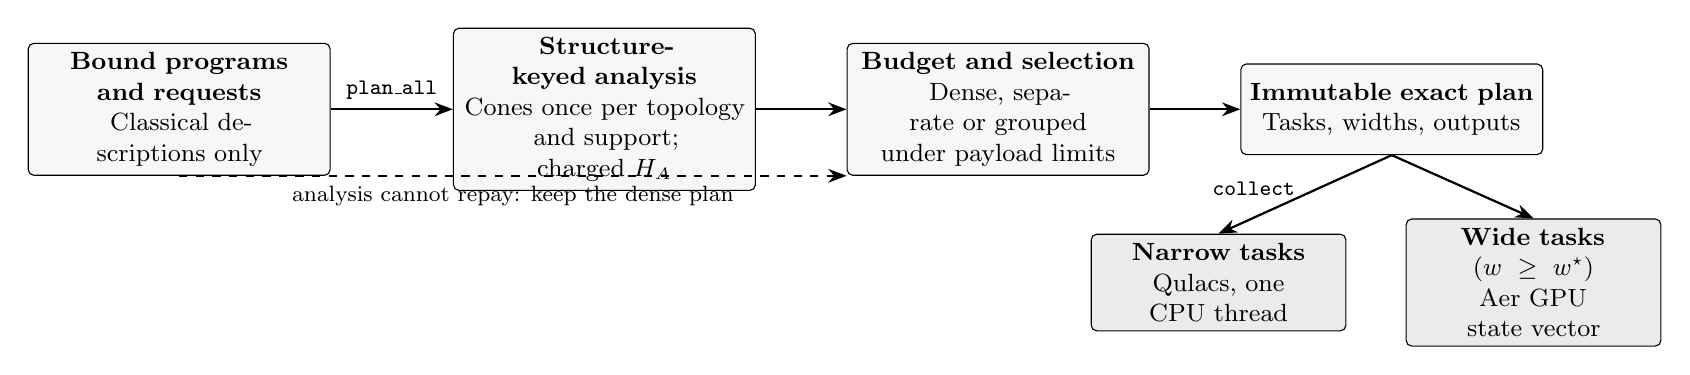
\begin{tikzpicture}[
 box/.style={draw, rounded corners=2pt, align=center, text width=3.6cm, minimum height=1.15cm, font=\small, fill=black!3},
 dev/.style={draw, rounded corners=2pt, align=center, text width=3.0cm, minimum height=0.9cm, font=\small, fill=black!8},
 arr/.style={-{Stealth}, thick}]
\node[box] (queries) at (0,0) {\textbf{Bound programs and requests}\\Classical descriptions only};
\node[box] (analysis) at (5.4,0) {\textbf{Structure-keyed analysis}\\Cones once per topology\\and support; charged $H_A$};
\node[box] (select) at (10.4,0) {\textbf{Budget and selection}\\Dense, separate or grouped\\under payload limits};
\node[box] (plan) at (15.4,0) {\textbf{Immutable exact plan}\\Tasks, widths, outputs};
\node[dev] (cpu) at (13.2,-2.2) {\textbf{Narrow tasks}\\Qulacs, one CPU thread};
\node[dev] (gpu) at (17.2,-2.2) {\textbf{Wide tasks} ($w\ge w^\star$)\\Aer GPU state vector};
\draw[arr] (queries) -- node[above,font=\footnotesize] {\texttt{plan\_all}} (analysis);
\draw[arr] (analysis) -- (select);
\draw[arr] (select) -- (plan);
\draw[arr] (plan.south) -- node[left,font=\footnotesize,yshift=2pt] {\texttt{collect}} (cpu.north);
\draw[arr] (plan.south) -- (gpu.north);
\draw[arr, dashed] (queries.south) |- node[below,font=\footnotesize,pos=0.75] {analysis cannot repay: keep the dense plan} (select.south west);
\end{tikzpicture}%
}
\caption{Planning and execution in \textsc{LazyQC}. Building requests allocates no simulator state. Planning extracts cones once per topology and observable support, keeps the dense plan when its predicted cost is below that of the analysis, and selects a feasible plan; the analysis charge $H_A$ is included in every end-to-end measurement. Collection allocates fresh states, running narrow tasks on the CPU and, when a wide backend is supplied, tasks of at least $w^\star$ qubits on a GPU. Everything in this execution path is exact. The opt-in approximate sensitivity extension is separate (Appendix~\ref{app:sensitivity}).}
\label{fig:architecture}
\end{figure*}

\subsection{Requests, plans and collection}
Programs are immutable descriptions of gates on wires, with rotations $R_P(\theta)=\exp(-i\theta P/2)$ and parameters that can remain symbolic until they are bound. A request pairs a bound program with a Pauli observable. Users build a list of requests, call \texttt{plan\_all} to obtain an immutable plan and execute it with \texttt{collect}. Planning is purely classical and allocates no simulator state. Collection allocates fresh states, evaluates the requested expectations and assembles them in request order. No numerical value survives a collection, so collecting a plan twice repeats the simulation instead of returning stale results.

A plan is a set of tasks, each of them a circuit on a contiguous local register together with the outputs it serves. The planner builds three candidate plans:
\begin{itemize}
\item \textbf{Full:} one task per distinct bound program, evaluating all of its outputs from the dense state. This is what a direct simulator does.
\item \textbf{Separate:} one cone task per output.
\item \textbf{Grouped:} one task per distinct cone circuit, shared by every output whose cone coincides with it, including outputs of different programs.
\end{itemize}
Sharing requires equality of the bound cone circuit, not of the observable or of the program. Two data examples or two shifted circuits that only differ outside an output's cone therefore share that output's task. The \textbf{separate} candidate is an internal ablation over our support-based cones, not a stand-in for Qiskit's commutation-aware \texttt{LightCone} pass; Section~\ref{sec:rq3} evaluates the actual Qiskit pass followed by Aer. Candidates whose widest task exceeds \texttt{max\_state\_qubits}, or whose state payload exceeds \texttt{max\_state\_bytes}, are rejected. The remaining ones are ranked by the work score
\begin{equation}
W=\sum_g 2^{m_g}\left(1+|C_g|+|\mathcal{G}_g|\right)
\label{eq:work-score}
\end{equation}
for task width $m_g$, gate count $|C_g|$ and output count $|\mathcal{G}_g|$, or by a calibrated execution-time model when one is supplied.

\subsection{Structure-keyed analysis}
Cone membership depends only on the wires each gate touches, never on its angle. The planner exploits this by keying its analysis on structure. For every distinct topology in the batch (the sequence of gate names and wires) and every distinct observable support, it computes the indices of the retained gates once. Each request then gathers the angles of those gates from its own bound program, and its grouping key is the pair formed by an interned cone shape and those angles. Equal keys mean equal cone circuits, exactly as comparing the gate sequences would, but the cost per request becomes proportional to the size of its cone instead of the size of the circuit. In a parameter-shift batch, where the base program and its $2P$ shifted versions share one topology, cones are computed once per output instead of once per request.

We verified the new analysis against the original per-request implementation on 60 randomized batches under all four strategies, 240 cases that mix shared and distinct topologies, equal programs held as distinct objects and identity observables. All candidate plans coincide task for task. On a 20-qubit hardware-efficient Jacobian batch with 3,220 requests, planning time fell from 262 to 26\,ms, which is what makes the gradient workloads of Section~\ref{sec:gradients} practical.

\subsection{Analysis budget}
Analysis can save at most the dense execution it replaces. When the dense plan is feasible and its predicted cost $\widehat T_{\mathrm{dense}}$ is below the predicted analysis cost $\widehat H$, no cone plan can repay the analysis, so \texttt{auto} keeps the dense plan without building cone candidates. We use
\begin{align}
\widehat T_{\mathrm{dense}}&=\sum_{p}\left(a_0+a_1G_p+\left(a_2G_p+a_3K_p\right)2^{n_p}\right),\\
\widehat H&=b_0+b_1\sum_r G_r,
\end{align}
where the first sum runs over the distinct programs $p$, with $n_p$ qubits, $G_p$ gates and $K_p$ requested outputs, and the second over the requests $r$. The coefficients were fitted by relative non-negative least squares on 312 seeded random circuits from 2 to 14 qubits, unrelated to the evaluation families. The fit gives $a_2\approx1.0$\,ns per amplitude-gate and $b_1\approx0.22\,\mu$s per request gate, with median relative errors of 14\% and 22\%. The rule is deliberately conservative, since it only skips analysis that could not pay even if every cone were free. It does not apply when the dense plan is infeasible, when a planning cache signals reuse or when a calibrated model is used, and \texttt{analysis="always"} restores exhaustive planning.

\subsection{Backends and placement}
A plan is independent of the simulator that executes it. \texttt{collect} accepts any backend able to lower a task, evolve it and return its expectation values. Besides single-thread Qulacs, the default, the prototype provides adapters for the CPU and GPU state vectors of Qiskit Aer and PennyLane Lightning, and for tensor-network contraction with quimb, which applies its own light-cone simplification to every local expectation. Only Qulacs executes the projector tasks of cut plans.

After planning, tasks can differ in size by many orders of magnitude. A narrow cone task of a few kilobytes takes microseconds on a CPU, much less than the fixed cost of running a circuit on a GPU, while a saturated full-width task benefits from the GPU's bandwidth. \texttt{collect} therefore also accepts a wide backend and a width threshold $w^\star$. Unitary tasks with at least $w^\star$ qubits run on the wide backend and the rest stay on the main one. Our wide backend is the GPU state vector of Qiskit Aer in double precision, and $w^\star=14$ is the per-task crossover measured on our host (Section~\ref{sec:method}). Placement happens after selection. The work score assumes a state vector and does not know which backends are available, so selecting plans, representations and devices jointly remains future work.

\subsection{Total cost and decision quality}
Let $\mathcal{F}$ be the feasible complete plans of a declared portfolio, and let an analysis policy $A$ generate a subset $\mathcal{G}_A\subseteq\mathcal{F}$ at cost $H_A$. With plan-specific setup $S(p)$ and per-collection cost $T_r(p)$ over $R$ collections, $C_R(p)=S(p)+\sum_{r=1}^R T_r(p)$, and the objective is
\begin{equation}
\min_{A,\,p\in\mathcal{G}_A}\;H_A+C_R(p).
\label{eq:planning-objective}
\end{equation}
For a selected plan $\hat p$, the excess cost over the best member of $\mathcal{F}$ decomposes into the analysis overhead $H_A$, a ranking regret $\Delta_{\mathrm{rank}}=C_R(\hat p)-\min_{\mathcal{G}_A}C_R$ and a coverage regret $\Delta_{\mathrm{cov}}=\min_{\mathcal{G}_A}C_R-\min_{\mathcal{F}}C_R$. If every prediction is within $d$ of the true cost, then $\Delta_{\mathrm{rank}}\le 2d$. Direct dense execution is the policy with $H_A=0$ and $\mathcal{G}_A=\{\text{full}\}$, and the analysis budget is the rule that falls back to it when $\widehat H$ exceeds the most that analysis could save. These are accounting identities rather than new mathematics, but they make explicit what every measurement below charges: the cost of deciding, and not only the cost of executing.

\subsection{Extensions}
The same planning boundary hosts several mechanisms that we evaluate as extensions. A joint batch planner searches request groups and exact CX channel cuts under fragment-width limits, using whole-program original, locally simplified and PyZX-verified rewrite variants as candidate circuits. It can replay a recorded structural plan for new bindings when the rewritten topology and the equality pattern of the bound preparations are unchanged. A persistent process pool executes independent tasks in parallel under an aggregate payload limit. Finally, an opt-in sensitivity profile admits zero-angle substitutions under per-output error budgets, using the conditional bound of Appendix~\ref{app:sensitivity}. An earlier version of the replay path could accept a template for a batch whose programs had different bindings, and a shortcut could select a candidate that did not cover every output. Both paths now validate the equality partition of bound preparations and the completeness of every candidate, with regression tests covering mixed bindings, duplicate outputs, constants, changed observables and rewrite-induced topology changes.

\section{Experimental Methodology}
\label{sec:method}
\subsection{Workloads}
The main comparison uses three generated QML circuit families, frozen together with their seeds in a manifest before any timing took place:
\begin{itemize}
\item \textbf{Hardware-efficient local:} data-encoding $R_X$ and trainable $R_Y$ rotations on every qubit, followed by two alternating sublayers of nearest-neighbour CX gates.
\item \textbf{QCNN-like local:} convolution and pooling blocks of $R_Y$, $R_X$ and two CX gates, applied with strides 1, 2, 4 and 4. It is a controlled QML-inspired circuit, not a canonical QCNN.
\item \textbf{Data re-uploading:} data $R_X$ and trainable $R_Y$ rotations on every qubit followed by a CX chain along the whole register, alternating direction. Its cones cover every wire after one layer, which makes it our saturation control.
\end{itemize}
All circuits have depth four. Outputs follow two patterns: $Z$ on every wire ($K=n$), which is the readout of a multi-output model, and $X$, $Y$ and $Z$ on wire 0 ($K=3$), the most favourable case for cones. Every configuration is evaluated on the two held-out circuit seeds of our earlier QML matrix (seed offsets 202 and 303), so none of the instances was used to design or tune the planner. For gradients, every $R_Y$ occurrence is an independent trainable parameter, which gives $P=4n$ parameters in the hardware-efficient and re-uploading families.

\subsection{Generalization studies}
\label{sec:generalization}
The main comparison is deliberately narrow, so three further studies test how far its conclusions travel. They run on the laptop, compare the planner on single-thread Qulacs with direct single-thread Qulacs, and use the same validation.
\begin{itemize}
\item \textbf{Held-out families.} Two families were added after the planner, its analysis budget and $w^\star$ had been frozen, so none of their timings informed any planner decision. The first is a MERA-like tree whose isometries join block heads at strides 1, 2, 4, and so on, with nearest-neighbour disentanglers on the block boundaries; its cones are narrow at depth two and saturated by depth eight. The second is the wiring of PennyLane's \texttt{StronglyEntanglingLayers}, general rotations followed by a CX ring of growing range, which saturates at every depth and is a public ansatz. We evaluate 8 to 20 qubits, depths 2, 4, 8 and 16, five seeds and three output patterns ($Z$ on every wire, $X$, $Y$ and $Z$ on one wire, and four scattered $Z$ outputs), 480 instances in all, each timed four times in each of two fresh interpreter sessions. The analysis plan, the strata and three decision criteria were frozen in a manifest before timing. Strata use only the planned grouped candidate: cones are narrow when its widest task covers less than half the register and saturated from 90\% on, and outputs share cones when grouping at least halves the number of separate tasks.
\item \textbf{Trained classifiers.} We trained 48 binary Iris classifiers with 4 and 8 qubits, a CX-ring and a nearest-neighbour brickwork ansatz, depths two and four, three data splits and two initializations, for 30 parameter-shift steps with every method. We also replay, without retraining, 15 classifiers trained in a separate study of encoding geometry with its own code base and simulator, on MNIST1D, EEG and PneumoniaMNIST data. These have 8 qubits, four data re-uploads of one \texttt{StronglyEntanglingLayers} layer, and 16 outputs ($Z_i$ and $Z_iZ_{i+1}$) that feed a trained linear head.
\item \textbf{Exhaustive reference on held-out families.} The 52-partition reference of RQ3, run on both new families at 6 and 8 qubits and depths two and four.
\end{itemize}

\subsection{Methods compared}
Table~\ref{tab:methods} summarizes the compared methods. We use the same engine as the planner (single-thread Qulacs) as the most direct reference, and the fastest engine we found for each hardware class as the strong reference. In a preliminary check on a 24-qubit re-uploading circuit, Qiskit Aer with gate fusion took 1.8\,s with 20 threads, against 8.7\,s for Qulacs with 20 threads and 12.4\,s for Qulacs with one, so Aer is our multi-threaded CPU reference. On the GPU, Aer was the fastest direct method from 24 qubits on (0.24 against 0.60\,s for Lightning GPU on the 24-qubit hardware-efficient circuits), while Lightning GPU was faster at 16 qubits and the two were close at 20, so we report both. Finally, to separate the benefit of planning from the choice of device, we ran the planner's tasks on each backend $B$ and compared them with direct execution on the same backend.

Two further baselines isolate the contribution from existing cone reduction and from the representation. First, the \emph{Qiskit LightCone + Aer} baseline runs Qiskit's actual commutation-aware pass independently for every output and shifted program, compacts the retained wires, and executes the resulting circuits in one Aer GPU job. We evaluate both one circuit per request and exact deduplication of identical reduced-circuit signatures across the complete batch. Pass execution, compaction, observable setup and deduplication are charged. This is deliberately not identified with our support-based \texttt{separate} candidate. Second, the beyond-device-memory study uses two stronger tensor-network comparators in addition to the legacy per-output quimb method: a reused-circuit quimb light-cone contraction and a global \texttt{CircuitMPS} with $\texttt{cutoff}=0$, prepared once per batch and shared by all outputs. The latter performs no bond truncation; its preparation and every requested expectation are included in its time. Claims about tensor-network representations rely on these shared baselines, not on the per-output strategy alone.

\begin{table}[!t]
\caption{Methods Compared. The Qiskit LightCone Baseline Uses the Actual Commutation-Aware Pass; the Global MPS Uses \texttt{cutoff}${}=0$ and Is Shared by Every Output in a Batch.}
\label{tab:methods}
\centering
\setlength{\tabcolsep}{2pt}
\footnotesize
\resizebox{\columnwidth}{!}{%
\begin{tabular}{llcl}
\toprule
Method & Engine & Threads & Role\\
\midrule
LazyQC & Qulacs & 1 & Planner, CPU collection\\
LazyQC+GPU & Qulacs, Aer GPU & 1 & Planner, wide tasks on GPU\\
Qulacs 1t & Qulacs & 1 & Direct, same engine\\
Aer CPU & Aer, fusion & 20 & Direct, strongest CPU\\
Aer GPU & Aer, fusion & 20 & Direct, strongest GPU\\
Lightning GPU & cuStateVec & 20 & Direct, second GPU\\
quimb & Tensor network & 20 & Direct, per-output light cones\\
Qiskit LC + Aer & LightCone, Aer GPU & 1 & Per-output cones, exact dedup\\
Reused quimb TN & Tensor network & 1 & Reused-circuit light cones\\
Exact global MPS & quimb \texttt{CircuitMPS} & 1 & Shared MPS, \texttt{cutoff}${}=0$\\
LazyQC on $B$ & As backend $B$ & 20 & All tasks on $B$\\
Aer GPU shift & Aer, fusion & 20 & Shift-rule gradients\\
Lightning adjoint & cuStateVec, CPU & 20 & Adjoint gradients\\
\bottomrule
\end{tabular}%
}
\end{table}

\subsection{Host and software}
All measurements run on one laptop: an Intel Core i7-13700H (6 performance and 8 efficiency cores, 20 hardware threads) with 31\,GB of RAM and an NVIDIA GeForce RTX 4060 Laptop GPU with 8\,GB (driver 595.84), under Linux 6.8 and Python 3.12. We use Qulacs 0.6.14, Qiskit 2.6.1 with qiskit-aer-gpu 0.18.0 on the CUDA 12 runtime, PennyLane 0.45.1 with Lightning 0.45.0 and custatevec-cu12 1.6.0, and quimb 1.15.0. The GPU baselines run in an isolated environment declared inline in the benchmark runners, so they never interfere with the project's locked dependencies. A laptop GPU is a modest device, so we repeated every GPU-dependent study on a cloud instance with an NVIDIA H100 PCIe of 80\,GB and 26 vCPUs of an Intel Xeon Platinum 8480+ (driver 570, CUDA 12.8), launched with SkyPilot from the same code and the same locked dependencies, with both thread passes on that host. Its CPU thread runs the planner about half as fast as the laptop's performance cores. Section~\ref{sec:discussion} reports what changes.

\subsection{Timing scope and fairness}
Every timing starts after the workload has been constructed. For \textsc{LazyQC} it includes planning and collection. Direct dense baselines receive prebuilt circuits, observables or tapes, are warmed up once per case, and are timed from state allocation to the last expectation value. They also get all 20 host threads, while \textsc{LazyQC} runs on one. Each of these choices favours the baselines. We run five repetitions per method and case at 12 to 20 qubits, three at 24 and 26, and two at 28, after a warm-up call. Methods run in a randomized order within each case. We report medians per case and geometric means over the two seeds; with two seeds per configuration, all ratios are descriptive. The single-thread and multi-threaded passes ran one after the other, so we repeated every 12- and 16-qubit case one hour later: the ratios between the fastest direct method and the planner agreed within a median of 7\% and at most 24\%, and no comparison changed side. The same check on the cloud host gave a median of 2.5\%, with the largest deviations at 16 qubits, where every method takes a few milliseconds.

The LightCone ablations use the same warm-up and randomized method order. They use three repetitions, except two for the 20-qubit Jacobian, and report geometric means over two circuit seeds. The original Qiskit DAG is prebuilt; every repetition includes all LightCone passes, wire compaction, expectation setup, optional deduplication and Aer execution. The exact global MPS and reused-circuit tensor-network timings have three repetitions per case and include preparation and all outputs. The beyond-device-memory planner runs have five. The 48-qubit depth-six and depth-eight cases use the same two held-out seeds and include CPU-only and GPU-placement planner variants. All these manifests were frozen before their respective timing runs.

\subsection{Validation}
Every timed result is checked. Within each case, all methods are compared with one reference, the planner's cone values or, when the cone saturates beyond 20 qubits, Aer GPU, and up to 12 qubits the reference is also checked against an independent matrix-free NumPy simulator. Beyond 28 qubits, where no state vector fits, planner values are compared with quimb local expectations computed by light-cone simplified tensor contraction. The global MPS is checked against the same values; the maximum discrepancy is $4.7\times10^{-12}$. Every LightCone baseline output, including every raw expectation in the parameter-shift batches, is checked against the planner's Qulacs result. Jacobians are compared with Lightning's adjoint Jacobians, and training-loss trajectories are compared across methods. The tolerance is $10^{-9}$ throughout.

\subsection{Placement threshold}
The threshold $w^\star$ was measured before the study by running full-state tasks of the re-uploading and hardware-efficient families through the \textsc{LazyQC} executor on both devices. Aer GPU pays a fixed cost of about 3.5 to 5\,ms per circuit, so it was 8 to 23 times slower than single-thread Qulacs at 8 to 10 qubits and twice as slow at 13. The ratio crossed one at 14 qubits (0.83 to 0.97) and reached 0.24 to 0.27 at 16. We fixed $w^\star=14$ in the manifest.

\section{Results}
\label{sec:evaluation}
We present the results following the four research questions. RQ1 maps where planning beats direct execution as the register grows, including beyond device memory. RQ2 repeats the comparison for gradient workloads and inside training loops. RQ3 measures how good the planner's decisions are and how much it pays to make them, and RQ4 collects the mechanisms that do not pay off. All simulated results passed validation: no value differed from its reference by more than $10^{-9}$. Hardware estimates are compared with exact values in Section~\ref{sec:rq4}.

\subsection{RQ1: Where does planning beat direct execution?}
\label{sec:rq1}
\begin{figure*}[!t]
\centering
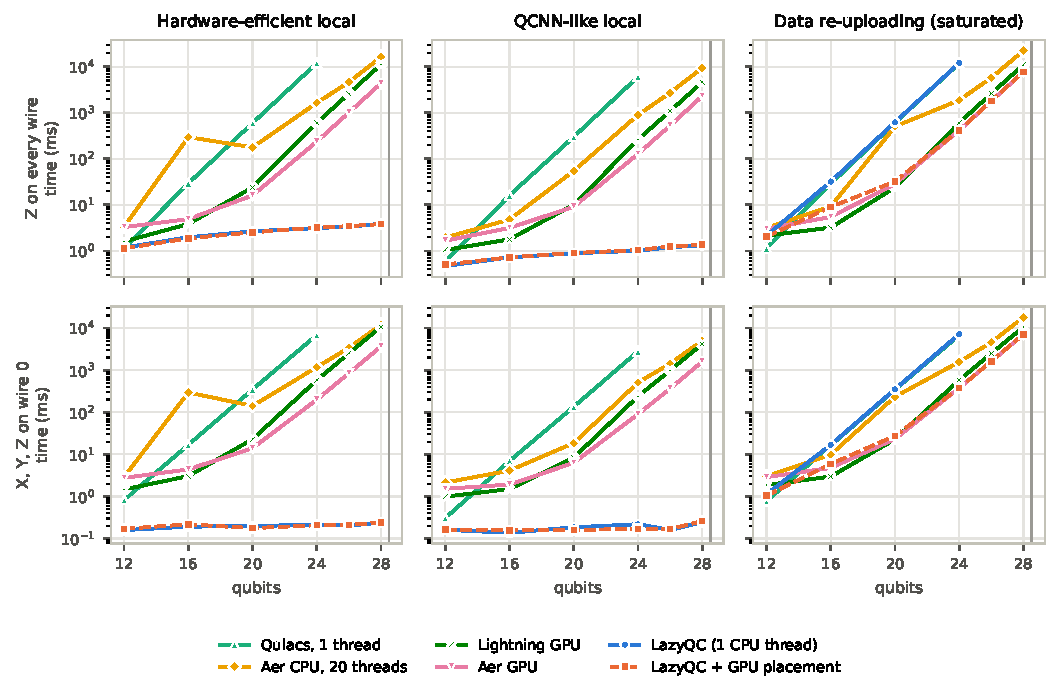
\includegraphics[width=\textwidth]{figures/direct_scaling.pdf}
\caption{Time to obtain every requested expectation value as the register grows, for the three circuit families (columns) and the two output patterns (rows). Each point is the median over repetitions of one case, averaged geometrically over two held-out seeds. The planner runs on one CPU thread and is charged with its analysis; direct methods receive prebuilt circuits and all 20 host threads. The vertical line marks the 28-qubit limit of the 8\,GB GPU in double precision. Aer CPU is slower at 16 than at 20 qubits on the hardware-efficient family, where synchronizing 20 threads dominates the small state. Lower is better.}
\label{fig:direct-scaling}
\end{figure*}

\begin{table}[!t]
\caption{Fastest Direct Method's Time Divided by the Planner's Time, with GPU Placement Enabled, by Number of Qubits. Values Above One Favour the Planner.}
\label{tab:rq1}
\centering
\setlength{\tabcolsep}{3pt}
\footnotesize
\resizebox{\columnwidth}{!}{\begin{tabular}{llrrrrrr}
\toprule
Family & Outputs & 12 & 16 & 20 & 24 & 26 & 28\\
\midrule
Hardware-eff. & $Z$, all & 1.00 & 2.05 & 6.34 & 73.3 & 295 & 1{,}137\\
Hardware-eff. & $X,Y,Z$, one & 4.84 & 14.0 & 79.5 & 960 & 3{,}987 & 15{,}279\\
QCNN-like & $Z$, all & 1.15 & 2.46 & 10.2 & 122 & 424 & 1{,}681\\
QCNN-like & $X,Y,Z$, one & 1.87 & 9.55 & 39.6 & 529 & 2{,}177 & 6{,}111\\
Re-uploading & $Z$, all & 0.56 & 0.36 & 0.74 & 1.00 & 1.00 & 1.00\\
Re-uploading & $X,Y,Z$, one & 0.74 & 0.50 & 0.83 & 1.01 & 1.00 & 1.00\\
\bottomrule
\end{tabular}
}
\end{table}

Fig.~\ref{fig:direct-scaling} shows the time needed to obtain every requested output as the register grows from 12 to 28 qubits, and Table~\ref{tab:rq1} gives the ratio between the fastest direct method and the planner. Three regimes stand out.

\textbf{Local families: work that no device can avoid.} For the hardware-efficient and QCNN-like families, the planner's time is almost flat. With $Z$ on every wire, it grows from 1.1 to 3.8\,ms (hardware-efficient) and from 0.5 to 1.4\,ms (QCNN-like) between 12 and 28 qubits, because every output keeps a cone of at most 10 and 8 qubits respectively, while every direct method doubles its cost with each added qubit. At 28 qubits the planner groups the 28 outputs of the hardware-efficient circuit into 14 tasks of at most 10 qubits and spends 1.4\,ms planning and 2.3\,ms collecting them, whereas the fastest direct method, Aer on the GPU, needs 4.35\,s. On a single CPU thread the planner ties with single-thread Qulacs at 12 qubits, and is 2.0 to 2.5 times faster than the fastest GPU method at 16 qubits (1.6 to 2.2 times in a later confirmation run), 6 to 10 times at 20, 73 to 122 times at 24 and 1,137 to 1,681 times at 28. When only the three Paulis on one wire are requested, a dense state serves fewer outputs and the margins grow further, from 1.9 to 4.8 times at 12 qubits to 6,111 to 15,279 times at 28. These ratios are large because the direct curves grow exponentially while the planner's do not. They are specific to our laptop GPU, but a faster GPU moves the direct curves down by a constant factor without changing their slope (Section~\ref{sec:discussion}).

\textbf{Saturated cones: hand the work over.} In the data re-uploading family every cone spans the whole register and the planner keeps the dense plan. On one CPU thread this costs what single-thread Qulacs costs plus the planner's overhead, which is visible at small widths (2.1 against 1.1\,ms at 12 qubits) and negligible at large ones (12.1 against 11.9\,s at 24 qubits). With width-based placement the dense task runs on the GPU instead. The fixed costs of planning, lowering the circuit and launching it make the planner 0.36 to 0.83 times as fast as the fastest GPU method between 16 and 20 qubits, but from 24 qubits on it matches direct Aer GPU within 0.6\% (0.997 to 1.006 times). The planner cannot speed up saturated work, but it does not need to make it slower either.

\textbf{Small circuits.} At 12 qubits every method takes about a millisecond and fixed costs dominate the comparison. The planner pays up to 0.6\,ms of analysis and 0.4\,ms of circuit lowering that direct methods with prebuilt circuits do not pay. It is still 1.15 to 4.8 times faster than the best direct method on three of the four local configurations, ties on the fourth and is 0.56 to 0.74 times as fast on the saturated control. The analysis budget of Section~\ref{sec:system} only skips analysis that could not pay even if every cone were free, so it rarely triggers at these sizes; RQ3 examines its effect on the cost of deciding.

\begin{table}[!t]
\caption{Held-Out Families on One CPU Thread: Planner Time over Direct Qulacs and Cross-Validated Selection Regret, Medians per Stratum at One Collection. The Five Top Strata Are Disjoint and Sum to 480; the Width Rows Break Down Their 405-Case Saturated Subset and Are Not Added Again. F, S and G Count the Full, Separate and Grouped Plans Chosen by \texttt{auto}.}
\label{tab:heldout}
\centering
\setlength{\tabcolsep}{3pt}
\footnotesize
\resizebox{\columnwidth}{!}{\begin{tabular}{lrlrr}
\toprule
Stratum & Cases & Auto choice & Auto/direct & CV regret\\
\midrule
\multicolumn{5}{l}{\emph{Disjoint family/cone strata (480 cases)}}\\
Tree, narrow, shared & 15 & G\,15 & 0.016 & 1.14\\
Tree, narrow, distinct & 10 & S\,10 & 0.003 & 1.07\\
Tree, intermediate & 50 & S\,35, G\,15 & 0.29 & 1.05\\
Tree, saturated & 165 & F\,100, G\,55, S\,10 & 1.12 & 1.06\\
Strongly ent., saturated & 240 & F\,170, G\,70 & 1.07 & 1.04\\
\midrule
\multicolumn{5}{l}{\emph{Width breakdown of the 405 saturated cases (overlapping rows)}}\\
Saturated, 8 qubits & 105 & F\,75, G\,30 & 1.82 & 1.41\\
Saturated, 12 qubits & 105 & F\,70, G\,35 & 1.24 & 1.13\\
Saturated, 16 qubits & 105 & F\,70, G\,30, S\,5 & 1.04 & 1.03\\
Saturated, 20 qubits & 90 & F\,55, G\,30, S\,5 & 1.00 & 1.00\\
\midrule
\multicolumn{5}{l}{\emph{All 480 cases (each counted once)}}\\
All held-out cases & 480 & F\,270, G\,155, S\,55 & 1.07 & 1.05\\
\bottomrule
\end{tabular}
}
\end{table}

\textbf{Unseen families.} The same regimes appear on the two families added after the planner was frozen (Table~\ref{tab:heldout}), here against direct single-thread Qulacs at depths 2 to 16. Where tree cones are narrow and outputs share them, the planner needs 0.016 times the direct time, about 60 times less. With narrow cones that outputs do not share it needs 0.003 times, and with intermediate cones 0.29 times. Where cones saturate, \texttt{auto} keeps the dense plan in two thirds of the cases and pays 1.07 to 1.12 times direct execution. That overhead is a matter of size rather than family: 1.82 times at 8 qubits, where a direct evolution takes 0.2\,ms, 1.24 at 12, 1.04 at 16 and 1.00 at 20. The fixed cost of deciding is visible only while the simulation itself takes about a millisecond.

\begin{table}[!t]
\caption{Same-Backend Comparison with $Z$ on Every Wire: Direct Execution Time Divided by the Time of LazyQC Running Its Tasks on the Same Backend, by Number of Qubits. Values Above One Favour LazyQC. Qulacs Uses One Thread; LazyQC on quimb Uses the Grouped Cone Plan. The quimb Row Is the Legacy Per-Output Comparator; Stronger Shared Tensor-Network Baselines Appear Below.}
\label{tab:backends}
\centering
\setlength{\tabcolsep}{3pt}
\footnotesize
\begin{tabular}{llrrrrr}
\toprule
Backend & Family & 12 & 16 & 20 & 24 & 28\\
\midrule
Qulacs, 1 thread & Hardware-eff. & 0.96 & 14.9 & 226 & 3{,}825 & n/a\\
Qulacs, 1 thread & QCNN-like & 1.24 & 22.3 & 339 & 6{,}030 & n/a\\
Qulacs, 1 thread & Re-uploading & 0.53 & 0.90 & 0.98 & 0.98 & n/a\\
Aer GPU & Hardware-eff. & 0.28 & 0.31 & 0.82 & 9.86 & 149\\
Aer GPU & QCNN-like & 0.19 & 0.26 & 0.71 & 6.76 & 95.8\\
Aer GPU & Re-uploading & 0.66 & 0.73 & 0.96 & 1.01 & 0.98\\
Lightning GPU & Hardware-eff. & 0.22 & 0.39 & 1.88 & 40.1 & 613\\
Lightning GPU & QCNN-like & 0.29 & 0.33 & 1.54 & 33.1 & 503\\
Lightning GPU & Re-uploading & 0.71 & 0.63 & 0.91 & 1.00 & 0.98\\
quimb & Hardware-eff. & 0.96 & 1.06 & 1.46 & 1.05 & 1.06\\
quimb & QCNN-like & 0.92 & 0.92 & 0.94 & 0.95 & 1.00\\
quimb & Re-uploading & 0.84 & 0.84 & 0.84 & 0.90 & 0.80\\
\bottomrule
\end{tabular}

\end{table}

\textbf{Planning on every backend.} The comparison above mixes two choices: whether to plan, and which device to use. To separate them, we ran the planner's tasks on each backend and compared them with direct execution on that same backend (Table~\ref{tab:backends}, 1,440 additional validated timings). On state-vector backends the benefit of planning grows exponentially with the register whatever the device: at 28 qubits, LazyQC on Aer GPU is 96 to 149 times faster than direct Aer GPU, and LazyQC on Lightning GPU 503 to 613 times faster than direct Lightning GPU. Below about 20 qubits, however, sending every small cone task to a GPU is slower than direct execution (0.19 to 0.39 times at 12 and 16 qubits), because each task pays the GPU's fixed launch cost. This is the regime in which width-based placement keeps them on the CPU, and a faster GPU makes it more important, not less: on the H100, LazyQC with every task on the GPU overtakes direct execution only at 28 qubits on Aer (1.8 to 3.0 times) and from 24 qubits on Lightning (2.0 to 2.5 times), whereas with narrow tasks kept on the CPU it wins from 16 qubits. With the legacy per-output quimb workflow, planning gains little (0.92 to 1.46 times with $Z$ on every wire, up to 2.4 times when several outputs share a wire). This row isolates reuse on one implementation; it is not evidence that tensor networks are generally slower, which the shared baselines below directly test. Across all configurations, LazyQC on single-thread Qulacs was the fastest way to evaluate the local families at every width (0.1 to 3.9\,ms), tying with direct Qulacs at 12 qubits on one of them. For the saturated family the best choice moved from Lightning GPU at 16 qubits (about 3\,ms) to quimb at 28 qubits, which evaluated all outputs in 4.4\,s against 7.8\,s for Aer GPU, and three outputs on one wire in 0.15 to 0.20\,s against 7.2\,s.

\begin{table*}[!t]
\caption{Total Batch Time in Milliseconds Beyond Device Memory, Geometric Means over Two Held-Out Seeds. For LazyQC, Width Is the Range of Reduced-Circuit Widths, Not the Logical Register Width $n$ Shown in the Column Headings. Exact MPS Includes Preparation with \texttt{cutoff}${}=0$ and Every Output; $\chi$ Is Its Maximum Bond Dimension. The Saturated Family Has No LazyQC Row Because the Planner Refuses It. Exact MPS Runs Have Three Repetitions and LazyQC Runs Five.}
\label{tab:memory-wall}
\centering
\setlength{\tabcolsep}{3pt}
\footnotesize
\resizebox{\textwidth}{!}{\begin{tabular}{lllrrrrrr}
\toprule
Method & Family & Outputs & Width / $\chi$ & 32 & 48 & 64 & 100 & 128\\
\midrule
LazyQC & Hardware-eff. & $Z$, all & 6--10 & 4.56 & 8.28 & 12.41 & 24.08 & 36.84\\
LazyQC & Hardware-eff. & $X,Y,Z$, one & 6 & 0.24 & 0.26 & 0.30 & 0.42 & 0.48\\
LazyQC & QCNN-like & $Z$, all & 2--8 & 1.65 & 2.53 & 4.00 & 8.11 & 12.64\\
LazyQC & QCNN-like & $X,Y,Z$, one & 8 & 0.20 & 0.19 & 0.21 & 0.27 & 0.27\\
\midrule
Exact MPS & Hardware-eff. & $Z$, all & $\chi{\le}32$ & 67.9 & 106.9 & 142.7 & 228.5 & 273.9\\
Exact MPS & QCNN-like & $Z$, all & $\chi{\le}8$ & 53.0 & 89.1 & 106.1 & 164.4 & 217.4\\
Exact MPS & Re-uploading & $Z$, all & $\chi{\le}16$ & 46.0 & 75.9 & 92.0 & 145.0 & 200.7\\
\midrule
\multicolumn{4}{l}{Dense state (bytes)} & $2^{36}$ & $2^{52}$ & $2^{68}$ & $2^{104}$ & $2^{132}$\\
\bottomrule
\end{tabular}
}
\end{table*}

\textbf{Beyond device memory: narrow cones versus a shared exact MPS.} Direct dense simulation stops at 28 qubits on our GPU, and at 32 qubits it would already need 64\,GiB. Table~\ref{tab:memory-wall} reports both logical width and the widths actually simulated. At 128 qubits with $Z$ on every wire, LazyQC takes 36.84\,ms for the hardware-efficient family, running 64 tasks of width 6--10, and 12.64\,ms for the QCNN-like family, running 112 tasks of width 2--8; planning accounts for 22.99 and 9.34\,ms respectively. With three outputs on one wire it stays below 0.5\,ms. All 44 planned cases in the expanded memory-wall study agree with quimb within $8.3\times10^{-14}$.

The exact global MPS is a much stronger baseline than independent per-output contractions. At 128 qubits it evaluates the same hardware-efficient and QCNN-like batches in 273.93 and 217.44\,ms, so LazyQC retains factors of 7.4 and 17.2 rather than the orders of magnitude suggested by a weak per-output comparison. Its maximum bond dimensions are 32 and 8. For the saturated data-re-uploading family, however, LazyQC refuses every case because no state-vector candidate satisfies the payload limit, whereas exact MPS succeeds: the 48-qubit depth-four batch takes 75.9\,ms and the 128-qubit batch 200.7\,ms. LazyQC's 20 refusals take 0.2 to 55\,ms. Thus the large-width claim is explicitly conditional: narrow-cone planning is faster on these local families; it is not dense 128-qubit simulation, and it is not a replacement for tensor contraction when cones saturate.

\begin{table}[!t]
\caption{Intermediate-Cone Hardware-Efficient Batches at 48 Logical Qubits, with $Z$ on Every Wire. All Entries Include Preparation or Planning and Every Output. The 24 Cone Tasks Have the Width Ranges Shown; a Full 48-Qubit Dense State Does Not Fit on the GPU. Times Are Geometric Means over Two Seeds, in Seconds.}
\label{tab:intermediate-cones}
\centering
\setlength{\tabcolsep}{3pt}
\footnotesize
\resizebox{\columnwidth}{!}{\begin{tabular}{llrr}
\toprule
Method & Width / $\chi$, $d=6/8$ & $d=6$ (s) & $d=8$ (s)\\
\midrule
LazyQC, CPU & 8--14 / 10--18 & 0.073 & 1.476\\
LazyQC, GPU placement & 8--14 / 10--18 & 0.074 & 0.171\\
Exact MPS & $\chi\leq128$ / $\chi\leq512$ & 0.275 & 5.578\\
quimb light-cone TN & -- & 3.270 & 5.566\\
\bottomrule
\end{tabular}
}
\end{table}

\textbf{The intermediate-cone boundary.} Table~\ref{tab:intermediate-cones} fills the missing regime around $w^\star$, reaching $w^\star<w\le28<n$ at depth eight. At depth six, cone widths are 8--14: LazyQC takes about 74\,ms on either placement, against 275\,ms for exact MPS and 3.27\,s for reused-circuit quimb contraction. At depth eight, widths grow to 10--18. CPU-only LazyQC takes 1.476\,s, while routing tasks at or above $w^\star=14$ to the GPU reduces the total to 171\,ms. Exact MPS and reused light-cone contraction take 5.578 and 5.566\,s. In this measured regime, placement contributes an 8.6-fold improvement over CPU-only cone execution, and the complete plan is 32.6 times faster than exact MPS. The result does not define a universal representation crossover: it uses one family at 48 qubits, but it demonstrates why plan selection and device placement must be evaluated separately.

\subsection{RQ2: Gradients and training}
\label{sec:gradients}
\begin{figure*}[!t]
\centering
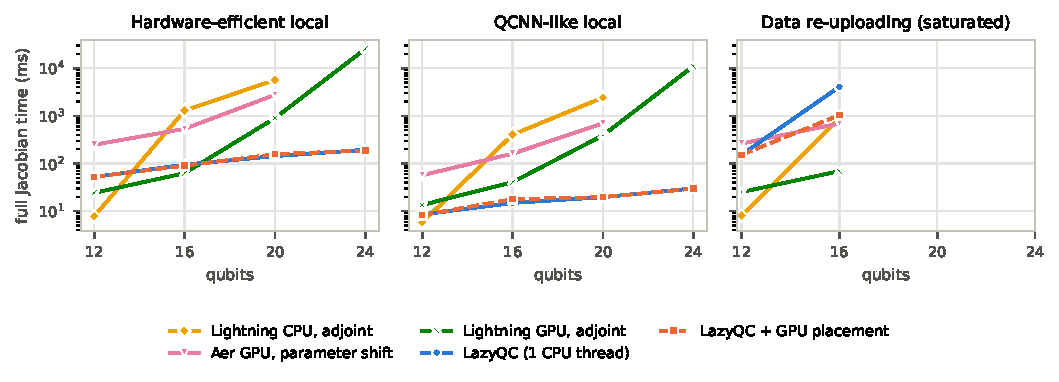
\includegraphics[width=\textwidth]{figures/gradient_scaling.pdf}
\caption{Time to obtain the full Jacobian of all $n$ outputs with respect to every trainable rotation, median per case and geometric mean over two seeds. The planner evaluates the base program and every $\pm\pi/2$ shift as one batch; Aer GPU runs every shifted circuit; Lightning uses adjoint differentiation. At 24 qubits the adjoint Jacobian with all observables exceeded GPU memory and was computed in chunks of eight observables. The saturated family was evaluated up to 16 qubits. Lower is better.}
\label{fig:gradients}
\end{figure*}

\begin{table*}[!t]
\caption{Full Jacobians: Trainable Rotations $P$, Distinct Tasks of the Planner, Structurally Zero Derivatives, and Median Time in Milliseconds per Method.}
\label{tab:jacobian}
\centering
\footnotesize
\setlength{\tabcolsep}{4pt}
\begin{tabular}{lrrrrrrrr}
\toprule
Family & $n$ & $P$ & Tasks & Zeros (\%) & LazyQC & Aer shift & L.\ GPU adj. & L.\ CPU adj.\\
\midrule
Re-uploading & 12 & 48 & 97 & 10 & 152 & 263 & 25 & 8.0\\
Re-uploading & 16 & 64 & 129 & 10 & 1{,}039 & 694 & 69 & 909\\
Hardware-eff. & 12 & 48 & 290 & 51 & 53 & 247 & 24 & 7.8\\
Hardware-eff. & 16 & 64 & 404 & 61 & 90 & 535 & 63 & 1{,}290\\
Hardware-eff. & 20 & 80 & 518 & 68 & 157 & 2{,}761 & 896 & 5{,}656\\
Hardware-eff. & 24 & 96 & 632 & 73 & 187 & n/a & 25{,}310 & n/a\\
QCNN-like & 12 & 22 & 102 & 74 & 8.3 & 57 & 13 & 5.8\\
QCNN-like & 16 & 32 & 158 & 80 & 18 & 161 & 41 & 403\\
QCNN-like & 20 & 38 & 181 & 84 & 20 & 701 & 390 & 2{,}422\\
QCNN-like & 24 & 48 & 237 & 86 & 30 & n/a & 11{,}048 & n/a\\
\bottomrule
\end{tabular}

\end{table*}

Gradient workloads multiply the number of requested circuits. Under the parameter-shift rule of Eq.~\eqref{eq:shift}, one Jacobian with respect to $P$ rotation occurrences requires the base circuit and $2P$ shifted ones, each with all $K$ outputs. They are also where a simulator has its strongest alternative: adjoint differentiation obtains all derivatives of an observable from about two passes over the state~\cite{jones2020adjoint}. We therefore compare the planner's shift-rule Jacobian with Aer GPU running every shifted circuit and with Lightning's adjoint method on the GPU and on the CPU (Fig.~\ref{fig:gradients} and Table~\ref{tab:jacobian}).

The object in this subsection is explicit: a full $K\times P$ Jacobian, with $K=n$ outputs and $(2P+1)K$ raw expectation requests. Table~\ref{tab:jacobian} reports $P$, the planner's distinct tasks, structurally zero entries and absolute times; Fig.~\ref{fig:gradients} compares methods computing that same object. Full Jacobians are useful for multi-output sensitivity, kernel construction and higher-order training methods, but are not required for an ordinary scalar-loss gradient step. The adjoint baseline is therefore configured to return the full Jacobian, including observable chunking when memory requires it; the cheaper scalar-loss vector-Jacobian product is evaluated separately below. The per-request Qiskit LightCone baseline for the raw expectation batch is reported in Table~\ref{tab:lightcone-ablation}.

\textbf{Shift rules meet cones.} The planner receives the $(2P+1)K$ requests of one Jacobian as a single batch. A shift that falls outside an output's cone leaves that output's cone circuit unchanged, so grouping evaluates it once together with the unshifted circuit, and the corresponding derivative comes out exactly zero without any special handling. These structural zeros are common: they are 51 to 73\% of the hardware-efficient Jacobian entries and 74 to 86\% of the QCNN-like ones. They rely on every rotation having its own parameter. When one parameter is shared by all rotations of a layer, a derivative is zero only if no occurrence of that parameter lies in the cone, and in a control at 8 and 12 qubits and depths two and four the median fraction fell from 0.49 to 0 on the hardware-efficient family and from 0.71 to 0.38 on the QCNN-like one. The planner does not run fewer circuits than direct parameter shift (632 tasks against 193 dense evolutions for the 24-qubit hardware-efficient Jacobian), but each of its tasks has at most 10 qubits, and structure-keyed analysis keeps planning at 44\,ms for 4,632 requests.

\textbf{Against adjoint differentiation.} At 12 qubits, CPU adjoint differentiation is the fastest way to obtain a Jacobian (7.8 against 53\,ms for the planner on the hardware-efficient family), and at 16 qubits GPU adjoint still leads on that family (63 against 90\,ms), while the planner is already 2.3 times faster on the QCNN-like one. From 20 qubits on the order reverses. The planner obtains the hardware-efficient Jacobian in 0.15\,s, against 0.90\,s for GPU adjoint and 2.8\,s for GPU parameter shift, and the QCNN-like one in 20\,ms against 0.39\,s. At 24 qubits the adjoint Jacobian with all 24 observables ran out of the GPU's 8\,GB, because the adjoint method keeps one state per observable during the backward pass. Computed in chunks of eight observables, it took 25\,s for the hardware-efficient family and 11\,s for the QCNN-like one, about 135 and 370 times the planner's 0.19 and 0.03\,s. Parameter shift on the GPU was the slowest option at every width, as expected from its $2P+1$ dense evolutions. For the saturated family the picture inverts: only 10\% of the derivatives are structural zeros, the planner evaluates all $2P+1$ circuits densely, and GPU adjoint is 15 times faster than the planner with GPU placement at 16 qubits. Cones help gradients exactly where they help forward passes.

\begin{table}[!t]
\caption{Ten Measured Gradient-Descent Steps on the Hardware-Efficient Family with $Z$ on Every Wire, Including Program or Tape Construction at Every Step.}
\label{tab:training}
\centering
\footnotesize
\begin{tabular}{rlrrr}
\toprule
$n$ & Method & Total (s) & Step (ms) & Final loss\\
\midrule
16 & Aer GPU, shift rule & 9.14 & 913 & 0.0841\\
16 & LazyQC, shift rule & 1.21 & 124 & 0.0841\\
16 & Lightning GPU, adjoint & 0.24 & 24 & 0.0841\\
20 & LazyQC, shift rule & 1.80 & 179 & 0.0760\\
20 & Lightning GPU, adjoint & 1.37 & 137 & 0.0760\\
24 & LazyQC, shift rule & 2.46 & 246 & 0.0909\\
24 & Lightning GPU, adjoint & 33.55 & 3355 & 0.0909\\
\bottomrule
\end{tabular}

\end{table}

\textbf{Training loops.} A training step does not need the full Jacobian, only the gradient of a scalar loss, which adjoint differentiation obtains as a single vector-Jacobian product. Table~\ref{tab:training} reports ten measured gradient-descent steps of a mean-squared loss over all outputs, each step paying for building the shifted programs or the tape, planning or executing, and updating the parameters. All methods follow the same loss trajectory, within $10^{-16}$ at every step. Here the planner competes with a cheaper quantity than before, and it loses at small widths: GPU adjoint is 5.0 times faster at 16 qubits and 1.3 times at 20. At 24 qubits the planner completes the ten steps in 2.5\,s against 33.6\,s, 13.6 times faster, because its steps grow with the number of outputs while every adjoint step doubles with each added qubit.

\subsection{RQ3: How good are the decisions, and what do they cost?}
\label{sec:rq3}
In the regime of RQ1 the decision is easy: the dense plan costs seconds and the cone plan milliseconds. It becomes delicate at small widths, where every candidate costs well under a millisecond and the analysis itself is a visible part of the total. We study that regime with the frozen QML matrix of our earlier work (240 cases at 8 and 12 qubits, five request patterns and eight repetitions per strategy) and its exhaustive reference, which times all 52 partitions of five same-state outputs, plus the dense plan, on 24 small cases. The held-out families of Section~\ref{sec:generalization} then test the same decisions on circuits the planner never saw. To separate the effect of the new planner from the drift of a laptop under sustained load, we ran the pre-study planner and the current one back to back in two rounds of alternating order. Collection times, whose code path did not change, agreed within 0.5\% between versions. Table~\ref{tab:rq3} summarizes the held-out cases.

\begin{table*}[!t]
\caption{Direct Comparison with Qiskit's Commutation-Aware \texttt{LightCone} Pass Followed by Aer GPU. S/D Is the Number of Circuits without/with Exact Reduced-Circuit Deduplication. All Analysis and Total Times Are Milliseconds and Include Lowering and Expectation Setup. LazyQC Uses \texttt{auto} Planning and Single-Thread Qulacs. Forward Rows Are Depth-Four Hardware-Efficient Circuits with $Z$ on Every Wire; Jacobian Rows Include the Base and All Shifted Programs. Values Are Geometric Means over Two Seeds.}
\label{tab:lightcone-ablation}
\centering
\setlength{\tabcolsep}{4pt}
\footnotesize
\resizebox{\textwidth}{!}{\begin{tabular}{llrrrrrr}
\toprule
Workload & Requests & LC tasks S/D & Lazy tasks & LC analysis & Lazy analysis & LC total & Lazy total\\
\midrule
Forward, $n=12$ & 12 & 12/12 & 6 & 27.0 & 0.58 & 38.7 & 1.57\\
Forward, $n=28$ & 28 & 28/28 & 14 & 77.5 & 1.72 & 103.6 & 4.28\\
Forward, $n=128$ & 128 & 128/128 & 64 & 849.5 & 25.61 & 974.9 & 39.21\\
Jacobian, $n=12$ & 1164 & 1164/504 & 290 & 2283.6 & 10.47 & 2762.8 & 63.64\\
Jacobian, $n=20$ & 3220 & 3220/896 & 518 & 7308.1 & 28.61 & 8221.8 & 152.19\\
\bottomrule
\end{tabular}
}
\end{table*}

\textbf{What changes relative to an existing LightCone pass.} Table~\ref{tab:lightcone-ablation} compares against the actual Qiskit implementation, not against our separate candidate as a proxy. Qiskit's commutation checks can produce smaller cones than our support traversal, while LazyQC's contribution is to cache structural analysis and plan sharing across the whole batch. In the forward study, exact deduplication does not reduce the Qiskit circuit count on these instances, whereas LazyQC groups each pair of preparations. At 128 qubits, Qiskit analysis takes 849.5\,ms against 25.61\,ms for LazyQC, and total times are 974.9 and 39.21\,ms. The Jacobian study exposes cross-program reuse: at 20 qubits, deduplication reduces 3,220 Qiskit circuits to 896, while LazyQC forms 518 tasks. Qiskit analysis takes 7.308\,s against 28.61\,ms, and totals are 8.222\,s against 152.19\,ms. At 12 qubits the corresponding totals are 2.763\,s and 63.64\,ms. These totals include different executors (Aer GPU for Qiskit and one-thread Qulacs for LazyQC) so the analysis columns are the cleanest isolation of the planning mechanism. The result supports a batch-planning contribution, not a claim of inventing cone reduction or of a better commutation analysis.

\begin{table}[!t]
\caption{Decision-Policy Ablation on 480 Held-Out Instances. Median and p90 Are Cross-Validated Total-Time Regret at One Collection. Narrow and Saturated Give Median Policy Time over Direct Qulacs. FP Selects a Cone Plan When Full Is Best (291 Cases); FN Selects Full When a Cone Plan Is Best (189 Cases). Simple Structural Selectors Pay the Same Analysis Cost as \texttt{auto}.}
\label{tab:policy-ablations}
\centering
\setlength{\tabcolsep}{2.5pt}
\footnotesize
\resizebox{\columnwidth}{!}{\begin{tabular}{lrrrrrr}
\toprule
Policy & Med. & p90 & Narrow & Saturated & FP & FN\\
\midrule
LazyQC \texttt{auto} & 1.055 & 1.534 & 0.004 & 1.095 & 26 & 5\\
Always full & 1.000 & 5.226 & 1.056 & 1.062 & 0 & 189\\
Always separate (per-output cone) & 2.797 & 7.424 & 0.004 & 3.144 & 291 & 0\\
Always grouped & 1.779 & 5.886 & 0.004 & 2.822 & 291 & 0\\
Width rule $w<n$ & 1.140 & 1.576 & 0.004 & 1.139 & 10 & 124\\
Width rule $2w\leq n$ & 1.165 & 1.694 & 0.004 & 1.139 & 0 & 154\\
Width rule $w\leq10$ & 1.152 & 3.188 & 0.004 & 1.150 & 95 & 119\\
\bottomrule
\end{tabular}
}
\end{table}

\textbf{Why a cost model instead of a width threshold.} Table~\ref{tab:policy-ablations} compares the frozen planner with simple alternatives using only the previously collected session timings. Among policies that exploit cones, \texttt{auto} has the lowest median cross-validated regret (1.055 against 1.140--1.165 for the three width-only rules), and its p90 is 1.534. Always keeping the full plan has median regret one because full is best in 291 of 480 instances, but its p90 is 5.226 and it misses every case where reduction helps: its median narrow-stratum time is 1.056 times direct, against 0.004 for the reducing policies. Always reducing is much worse on saturated cases (2.822--3.144 times direct). The error counts expose the trade-off rather than hiding it: the $w<n$ rule has fewer false-positive reductions than \texttt{auto} (10 against 26), but 124 false negatives against five. Thus \texttt{auto} is not uniformly optimal, but its total-cost score makes materially better batch decisions than any tested single width rule.


\begin{table}[!t]
\caption{Cost of Deciding at Small Widths: Pre-Study and Current Planner, Held-Out Cases, Ranges over the Two Interleaved Rounds.}
\label{tab:rq3}
\centering
\setlength{\tabcolsep}{3pt}
\footnotesize
\begin{tabular}{lrr}
\toprule
Quantity & Pre-study & Current\\
\midrule
Auto planning time (relative) & 1 & 0.57\\
Forced dense planning time (relative) & 1 & 0.25\\
Median auto total, 8 / 12 qubits (ms) & 0.72 / 1.22 & 0.55 / 0.95\\
Median overhead over best forced (ms) & 0.18 / 0.14 & 0.19 / 0.07\\
Auto / best forced, per request pattern & 1.19--1.35 & 1.18--1.50\\
\midrule
\multicolumn{3}{l}{Exhaustive reference: auto relative to the fastest partition}\\
\quad execution only & 1.17--1.21 & 1.17--1.18\\
\quad total, one collection & 3.09--3.25 & 2.80--2.85\\
\quad total, five collections & 1.56--1.62 & 1.49--1.52\\
\quad total, 32 collections & 1.23--1.27 & 1.22--1.23\\
\bottomrule
\end{tabular}
\end{table}

\textbf{The decisions did not change; deciding got cheaper.} The structure-keyed analysis is equivalent to the original one, and the analysis budget did not trigger on any of these cases, so both planners selected the same plans. The automatic plan's execution stays within 1.17 to 1.21 times the fastest of the 52 measured partitions, a figure that already includes the optimistic bias of taking a minimum over 52 noisy candidates. What changed is the cost of deciding: automatic planning takes 0.57 times its previous time, and the median total time fell from 0.72 to 0.55\,ms at 8 qubits and from 1.22 to 0.95\,ms at 12. Charged against a single collection, the automatic plan now costs 2.8 times the fastest partition's execution instead of 3.1 to 3.2 times, and after five collections 1.5 times instead of 1.6.

\textbf{Small widths remain the planner's weak spot.} Against the best forced policy, automatic planning still costs 1.18 to 1.50 times as much at these widths, slightly more than before for some request patterns. The reason is instructive: the forced dense plan became four times cheaper to plan as well, because it also uses structure keys, so the reference moved faster than the automatic plan did. In absolute terms the median overhead is 0.07 to 0.19\,ms, with a 90th percentile of about half a millisecond. That is negligible next to any of the RQ1 savings, but not next to a simulation that itself takes a millisecond.

\begin{table}[!t]
\caption{Exhaustive Reference: Automatic Plan Relative to the Fastest of the 52 Partitions and the Dense Plan, Geometric Means. Execution Regret Is the Product of Ranking Regret, against the Best Candidate the Planner Generated, and Coverage Regret, of that Candidate against the Best Partition.}
\label{tab:regret}
\centering
\setlength{\tabcolsep}{3pt}
\footnotesize
\resizebox{\columnwidth}{!}{\begin{tabular}{lrrrrr}
\toprule
Split & Cases & Execution & Ranking & Coverage & Total, $R{=}1$\\
\midrule
Development seeds & 12 & 1.16 & 1.12 & 1.03 & 2.95\\
Held-out seeds & 12 & 1.14 & 1.09 & 1.05 & 2.89\\
Held-out family: tree & 8 & 1.38 & 1.29 & 1.06 & 2.82\\
Held-out family: strongly ent. & 8 & 1.06 & 1.03 & 1.02 & 2.62\\
\bottomrule
\end{tabular}
}
\end{table}

\textbf{Decisions on unseen families.} On the held-out families, we estimate selection regret by cross-validation: the best forced plan is chosen on one interpreter session and evaluated on the other, so a noisy minimum cannot flatter the reference. Its median is 1.055 at one collection (bootstrap 95\% interval 1.035 to 1.073, against 1.061 in-sample), and 1.01 after eight collections. \texttt{auto} chose the plan with the lowest pooled time in 418 of the 480 instances. The three criteria frozen before timing all hold: at least a 10\% gain over direct execution where cones are narrow and shared (median 0.016, interval 0.002 to 0.24), at most 10\% selection regret overall (1.055), and at most a 10\% loss where cones saturate (1.095, interval 1.066 to 1.122). Two caveats limit what this shows. The last criterion passes on its median while its interval crosses the threshold, and the first rests on 15 instances of one family and one output pattern. The regret tail sits where Table~\ref{tab:heldout} puts the overhead, with a median cross-validated regret of 1.41 at 8 qubits and 1.00 at 20.

\textbf{Ranking, not coverage.} Section~\ref{sec:system} splits the excess cost of a decision into analysis overhead, ranking regret and coverage regret, and the exhaustive reference measures the last two (Table~\ref{tab:regret}). Coverage regret, the price of partitions the bounded search never builds, is 1.02 to 1.06 in every split, including both unseen families. Nearly all of the execution regret is ranking. On small tree circuits the planner prefers a cone plan when the dense plan is up to 1.9 times faster, which gives a ranking regret of 1.29. The work score of Eq.~\eqref{eq:work-score} explains why: every term grows with $2^{m_g}$, so the score has no constant for the fixed cost of lowering and launching a task, which dominates below a millisecond. On these cases, analysis is 52 to 63\% of the automatic plan's time at one collection. A per-task constant in the score, or a size guard that skips analysis for tiny batches, would target this tail. Either would be a new rule that must be evaluated on fresh instances, so we leave it to future work.

\textbf{When the budget matters.} The budget is designed for batches whose analysis would exceed the dense execution, which never happens in the QML matrix. Hamiltonian averaging on small circuits is such a case: a 6- to 12-qubit hardware-efficient ansatz with linear CX chains and 16 to 128 overlapping local Pauli terms, the shape of a small-molecule energy evaluation. Over 540 validated timings, the budget skipped analysis in 8 of the 12 configurations, all up to 10 qubits, and the automatic plan then matched the forced dense plan (1.04 times in geometric mean), while always analysing cost 1.69 times as much. In the other four, the analysis was predicted to be affordable, ran, and found only saturated cones, so automatic planning cost 1.3 to 1.8 times the dense plan with or without the budget. A cheap early test for cone saturation would recover these cases, and is a natural next refinement.

\textbf{Reusing the analysis across a trajectory.} For the joint planner, whose search is much more expensive than the cone analysis, structural replay reuses group and cut decisions across parameter points when the rewritten topology and the equality pattern of bound preparations are unchanged. On the QML replay probe (24 held-out trajectories of six parameter points at 8 and 12 qubits, with template creation charged once), replay hit the template every time and reduced median planning time from 7.99 to 1.70\,ms for shared-bound trajectories and from 16.20 to 3.85\,ms for shift-pair trajectories. The whole trajectory became 2.37 times cheaper in geometric mean, with every replayed output within $2.9\times10^{-15}$ of an independent NumPy reference.

\subsection{RQ4: What does not pay off}
\label{sec:rq4}
The previous results describe the regime where planning wins. Equally important for practitioners is where it does not, because a planner that is enabled by default must lose little there. We group the evidence by mechanism.

\textbf{Parallel workers for small tasks.} Cone reduction leaves little for workers to accelerate. On the held-out 12-qubit, depth-four QML probe (24 cases with fixed execution graphs and 1,152 validated collections), four workers reduced the summed collection time by 12\%, but per case they were 1.52 to 1.64 times slower than serial execution and won only 6 to 8 of the 24 cases. After charging one pool start-up and shutdown, the whole probe took 0.998 times the serial time, and two workers cost 1.32 times. Workers paid off only on wide independent components, with 3.18 to 3.28 times warm speedup for eight 16-qubit components on four workers (Appendix~\ref{app:parallel}). Planning and parallelism compete for the same slack: once the planner has shrunk the tasks, there is little left to distribute, which is also why we do not consider distributed execution part of the contribution.

\textbf{Exact cutting at small widths.} Joint cut selection does reduce unique fragment experiments, from 148 to 67 on a QAOA path, and repeated collections repay its search after 18 to 21 calls (Appendix~\ref{app:earlier}). None of these comparisons beats dense execution while the dense state fits, though: ten dense collections of a six-qubit path took 1.06\,ms against 389\,ms for the joint cut plan. With $10^k$ exact branch combinations for $k$ cuts, cutting is a fallback for cones that exceed the payload limit by a few qubits rather than an accelerator.

\textbf{ZX rewrites.} In a 12-qubit pilot with 64 Pauli terms, verified ZX rewriting spent 199\,ms of search to produce the same 11 groups as no rewriting, and in the cutting fixtures both policies selected original-circuit variants. We have not isolated a positive contribution of rewriting to plan cost.

\textbf{Quantum hardware.} Plans are ordinary circuits and can be submitted to hardware, but the trade-off changes there, because a QPU returns every same-basis output of a circuit from one set of shots. On IQM Garnet, with 20 same-state $Z$ outputs of a 20-qubit hardware-efficient circuit and 100 shots per circuit, the full circuit used one circuit and 0.70\,s of station execution time, while grouped cones needed 10 circuits and 1.06\,s, and separate cones 20 circuits and 1.40\,s. Cones can only help when few outputs are requested or when they need different measurement bases. We tested that case with $X$ and $Z$ on two wires of the same circuit, two seeds, 300 shots per output in every plan and a randomized plan order. A fair accuracy comparison needs every plan to read its outputs on the same physical qubits. Garnet's coupling graph has no 20-qubit Hamiltonian path, but it has a 19-qubit path that starts at the two output qubits, so we mapped the logical wires of every plan onto it. Cone circuits then need no routing, and only the full circuit routes its last wire, far from the outputs. With this placement, grouped cones ran in 0.56 times the full circuit's execution window at equal shots on both seeds, and in 0.69 to 0.85 times the window of separate cones with half their shots, using 14 two-qubit gates per circuit against 88. No accuracy difference between plans was resolved: the mean absolute error against exact values was 0.054 to 0.062, and every paired difference had a bootstrap interval spanning zero. An earlier run that moved the outputs into place with terminal SWAPs had found grouped cones less accurate than separate ones, and the repeat traces that deficit to their six extra SWAPs. Earlier two-output pilots with automatic and identity layouts pointed the same way but confounded placement. Two seeds on one device with sequential jobs say nothing about queues or scheduling, so the hardware evidence remains exploratory. IonQ's noisy simulator shows the same pattern in processing time (17\,s for full 20-qubit jobs against 1\,s for width-six cone jobs), which is not a hardware measurement.

\begin{table}[!t]
\caption{Trained Classifiers on One CPU Thread: Median Time over Direct Qulacs. Iris Rows Time Complete 30-Step Training Runs, Replayed Rows Time Inference Batches of 64 Examples Including Setup. F and G Denote the Full and Grouped Plans Chosen by \texttt{auto}.}
\label{tab:trained}
\centering
\setlength{\tabcolsep}{3pt}
\footnotesize
\resizebox{\columnwidth}{!}{\begin{tabular}{lrlrr}
\toprule
Models & $N$ & Auto choice & Auto/direct & Grouped/direct\\
\midrule
Iris, brickwork, 4 qubits & 12 & F, G & 1.77 & 1.64\\
Iris, brickwork, 8 qubits & 12 & F & 1.34 & 1.42\\
Iris, ring, 4 qubits & 12 & F & 1.81 & 2.19\\
Iris, ring, 8 qubits & 12 & F & 1.37 & 3.54\\
\midrule
MNIST1D, 8 qubits & 5 & F & 1.23 & 5.59\\
EEG, 8 qubits & 5 & F & 1.27 & 5.66\\
PneumoniaMNIST, 8 qubits & 5 & F & 1.24 & 5.49\\
\bottomrule
\end{tabular}
}
\end{table}

\textbf{Small trained classifiers.} Trained models at the widths where we could train them do not benefit (Table~\ref{tab:trained}). For each of the 48 Iris classifiers, direct Qulacs was faster than every planned method, by 1.3\% in the closest case, and \texttt{auto} cost 1.34 to 1.81 times as much over a complete training run. Each step changes the parameters and therefore builds a new plan, and the circuits are too small for cones to repay it. The brickwork ansatz keeps cones local, four of eight qubits at depth two, yet grouped cones still cost 1.42 to 1.64 times direct execution. The 15 replayed classifiers saturate their cones with four re-uploads of a CX ring. \texttt{auto} kept the dense plan for all of them, within 2\% of the forced dense plan, and still cost 1.23 to 1.27 times direct Qulacs, because \textsc{LazyQC} lowers native circuits at every collection. Grouped cones, which ignore the saturation, cost 5.5 to 5.7 times. Replaying these models also checks the circuit translation against a different simulator and code base: all 3,300 saved test predictions were reproduced exactly. The planning cache cannot help such inference either, since new data change the bindings that its keys include.

\textbf{Approximation without structural change.} The opt-in sensitivity mechanism of Appendix~\ref{app:sensitivity} pays off only when an admissible substitution changes the structure of the plan. On constructed 16-qubit circuits with weak bridges it halves the maximum width and gives 2.89 to 3.57 times speedup over eight fully charged collections, while a connected control and all eight-qubit fixtures regress once profiling is charged.


\section{Discussion and Limitations}
\label{sec:discussion}
\subsection{Planning and acceleration compose}
The central observation of this study is that a planner and a GPU attack different factors of the same cost. Direct dense simulation of a batch performs roughly $\sum_p G_p 2^{n_p}$ amplitude-gate updates. A GPU lowers the time of each update, while the planner changes how many updates are needed: it replaces $2^{n}$ by $2^{w}$ for every distinct cone and the number of prepared states by the number of distinct cone circuits. When cones are narrow, the second factor wins by an exponential margin and the GPU has nothing left to do: at 28 qubits the planner, on one CPU thread, spends 3.8\,ms on the laptop and 4.6 to 6.8\,ms on the cloud host, where Aer spends 4.35\,s on the laptop GPU and 0.39\,s on an H100. When cones saturate, there is nothing to remove, and the right behaviour is to hand the work to the fastest device, which is what width-based placement does: on our saturated control, it matched direct execution on the laptop GPU within 0.6\% from 24 qubits on, and on the H100 at 28. The two techniques are therefore complements rather than competitors, and the question a planner should answer is not whether it can replace the GPU but which part of the requested work needs it.

The 48-qubit intermediate-cone cases make this separation concrete. At depth eight the planner's tasks are 10--18 qubits wide: too wide for efficient serial CPU execution, but small enough for the GPU even though a full 48-qubit state is impossible. GPU placement reduces total time from 1.476\,s to 171\,ms without changing the selected plan. This is the value of treating plan choice and device placement as separate decisions.

\subsection{What a datacenter GPU changes}
\begin{table}[!t]
\caption{Fastest Direct Method's Time over the Planner's, Each Measured Within One Host: the Laptop RTX 4060 (Lap.) and a Cloud H100 PCIe (Rem.), by Number of Qubits.}
\label{tab:remote}
\centering
\footnotesize
\resizebox{\columnwidth}{!}{\begin{tabular}{llrrrrrrrr}
\toprule
 & & \multicolumn{2}{c}{16} & \multicolumn{2}{c}{20} & \multicolumn{2}{c}{24} & \multicolumn{2}{c}{28}\\
\cmidrule(lr){3-4}\cmidrule(lr){5-6}\cmidrule(lr){7-8}\cmidrule(lr){9-10}
Family & Outputs & Lap. & Rem. & Lap. & Rem. & Lap. & Rem. & Lap. & Rem.\\
\midrule
Hardware-eff. & $Z$, all & 2.05 & 1.86 & 6.34 & 1.65 & 73.3 & 8.09 & 1{,}137 & 57.0\\
Hardware-eff. & $X,Y,Z$, one & 14.0 & 11.8 & 79.5 & 31.1 & 960 & 98.3 & 15{,}279 & 1{,}203\\
QCNN-like & $Z$, all & 2.46 & 1.64 & 10.2 & 3.98 & 122 & 17.0 & 1{,}681 & 119\\
QCNN-like & $X,Y,Z$, one & 9.55 & 6.88 & 39.6 & 17.5 & 529 & 57.7 & 6{,}111 & 592\\
Re-uploading & $Z$, all & 0.36 & 0.22 & 0.74 & 0.25 & 1.00 & 0.64 & 1.00 & 0.95\\
Re-uploading & $X,Y,Z$, one & 0.50 & 0.27 & 0.83 & 0.24 & 1.01 & 0.69 & 1.00 & 0.97\\
\bottomrule
\end{tabular}
}
\end{table}
Our main GPU is a laptop device with 8\,GB of memory and about 256\,GB/s of memory bandwidth. We therefore repeated every GPU-dependent study on a cloud host with an NVIDIA H100 PCIe of 80\,GB, measuring every planner/direct ratio within that host (Table~\ref{tab:remote}). The H100 ran the 28-qubit dense circuits 11 to 18 times faster than the laptop GPU, while the host's CPU thread ran the planner about half as fast as the laptop's. The result is the shift we expected rather than a change of regime. For the local families the margins at 28 qubits shrink by a factor of 10 to 20, to 57 to 119 times with $Z$ on every wire and 592 to 1,203 times with three outputs on one wire, but the planner still wins from 16 qubits (1.6 to 1.9 times) and its advantage still grows exponentially. Gradient crossovers move by a few qubits. The full hardware-efficient Jacobian still favours the planner from 20 qubits, but by 1.3 rather than 5.7 times there and by 12 rather than 135 times at 24 qubits, where the 80\,GB device also avoids the out-of-memory failure of the adjoint method. The ten-step training loop ties with GPU adjoint at 24 qubits instead of being 13.6 times faster. On the saturated family the planner's fixed costs weigh more against a faster GPU, and placement reaches parity only at 28 qubits (0.95 to 0.97 times, against 0.22 to 0.69 between 16 and 24). An H100 also moves the memory wall from 28 to about 32 qubits in double precision, which we did not explore.

\subsection{Where the incremental contribution lies}
The stronger baselines change the interpretation of the results. Qiskit's LightCone pass already performs commutation-aware reduction, and a global MPS already shares one tensor representation across outputs. Consequently, neither cone reduction nor multi-output reuse can be the paper's novelty claim. The measured increment is the planning layer: structure-keyed analysis across a shift batch, exact grouping of the resulting bound preparations, an explicit decision about when analysis pays, and placement of the remaining tasks. The LightCone ablation isolates this layer by charging every Qiskit pass and deduplication step; the MPS experiments show that the resulting plan still has to compete with a fundamentally different representation.

The same experiments also bound that contribution. Qiskit's commutation analysis can remove gates our support traversal keeps. Exact MPS evaluates the saturated 48-qubit depth-four batch in 75.9\,ms, while LazyQC refuses it. At 128 qubits, the local-family advantage over exact MPS is 7.4--17.2 times, not the three-orders-of-magnitude margin against direct dense execution. A defensible claim is therefore not ``cones are faster than tensor networks,'' but ``a cost-aware batch planner can choose and reuse reduced state-vector work effectively in measured regimes, and its decisions can be evaluated independently of the backend.''

\subsection{Limitations}
Our conclusions hold for the workloads we measured, and several of their features favour or disfavour cones in ways a reader should keep in mind:
\begin{itemize}
\item \textbf{Workloads.} Every direct GPU result comes from the main comparison: generated families of depth four on two held-out seeds. The generalization studies widen this to two unseen families at depths 2 to 16 with five seeds and to 63 trained classifiers, but only on one CPU thread, at up to 20 qubits, and the trained models have at most 8 qubits. The LightCone comparison covers the hardware-efficient family with $Z$ outputs, and the shared-MPS study covers the generated families at depths four, six and eight. Trained models wide enough for cones to matter remain untested.
\item \textbf{Conservative cones.} The support-based traversal keeps gates that overlap but commute with the propagated observable. Qiskit's commutation-aware pass can produce narrower cones; implementing a commutation-aware analysis while retaining structure-keyed batch reuse is future work.
\item \textbf{Comparison scope.} QuWARP is a related shared-prefix planner, not a head-to-head baseline: our implementation and artifacts do not reproduce its Qrack execution surface or typed continuations. Pauli-propagation methods are discussed but not benchmarked. Tensor-network conclusions are limited to the tested quimb contraction and exact MPS configurations, not every contraction strategy or approximate tensor method.
\item \textbf{Two hosts.} Most measurements come from one laptop, and the direct GPU studies were repeated on one cloud host with an H100. Absolute times and the placement threshold depend on the host, and the analysis-budget coefficients and $w^\star$ were fitted on the laptop. The new LightCone and tensor-network studies ran on the laptop.
\item \textbf{Fixed per-task costs.} The work score has no per-task constant, so below a millisecond it can prefer a cone plan that the dense plan beats (RQ3). \textsc{LazyQC} also lowers native circuits at every collection, which costs about 25\% against a prebuilt direct circuit at 8 qubits, and its planning cache keys on parameter bindings, so it cannot amortize analysis across inference batches with new data. The policy ablation diagnoses this issue but does not tune a replacement on the held-out cases.
\item \textbf{Placement after selection.} The planner chooses a plan with a CPU-oriented score and only then places wide tasks on the GPU. Selecting plans, representations and devices jointly, or batching many narrow cone tasks into one GPU kernel, could change decisions near the crossover.
\item \textbf{Exact expectations.} The core comparisons evaluate exact expectation values. Shot noise, noisy simulation and the statistics of measurement grouping are outside the evaluated scope, and the hardware probes of Section~\ref{sec:rq4} are exploratory, with two seeds on one device. The optional sensitivity approximation is not part of the exact planner and its bound assumes an explicit numerical allowance rather than outward-rounded floating-point certification.
\end{itemize}

\section{Conclusions}
\label{sec:conclusion}
We have presented \textsc{LazyQC}, a cost-aware batch planner for observable-specific quantum expectation workloads. Its contribution is not causal-cone reduction itself, but the decision layer above existing reduction and simulation mechanisms: structure-keyed cone analysis, exact grouping of bound reduced circuits across outputs and parameter shifts, an analysis-aware dense fallback, and width-based CPU/GPU placement. The core execution path is exact and every reported end-to-end time includes planning.

Direct comparisons isolate that contribution. On a 20-qubit, 3,220-request Jacobian batch, per-request Qiskit LightCone reduction with exact deduplication and Aer execution takes 7.308\,s of analysis and 8.222\,s in total, against 28.61\,ms and 152.19\,ms for LazyQC. On 480 held-out instances, the frozen planner obtains median cross-validated regret 1.055, compared with 1.140--1.165 for the tested width-only rules, while explicit false-positive and false-negative counts show where its decisions still fail. Against direct dense GPU execution, the planner is 1.6--2.5 times faster at 16 qubits and 57--119 times faster than an H100 at 28 on the stated depth-four local families with $Z$ on every wire. Full-Jacobian and scalar-loss training results remain separate tasks with separate baselines.

Strong tensor-network baselines narrow the claim in a useful way. At 128 logical qubits, LazyQC evaluates the local batches in 12.64--36.84\,ms using cone widths 2--10, against 217.44--273.93\,ms for exact global MPS. In the 48-qubit depth-eight intermediate-cone case, GPU placement lowers total time from 1.476\,s on the CPU to 171\,ms, against 5.578\,s for exact MPS. Conversely, exact MPS evaluates saturated cases that the state-vector planner refuses, small trained classifiers do not repay planning, and Qiskit's commutation-aware cones can be narrower than ours. These are boundaries of the contribution, not exceptions to hide.

The next technical steps follow directly from these boundaries: commutation-aware cones with structure-keyed reuse, a per-task fixed-cost term evaluated on fresh workloads, joint selection of plan and device, and principled handoff between state-vector and tensor-network representations. An immutable public artifact tying every reported table and figure to its frozen raw observations remains a submission requirement.


\clearpage
\appendices
\section{Approximation Under Per-Output Error Budgets}
\label{app:sensitivity}
Exact planning never changes an answer. This appendix describes the one opt-in mechanism that does: replacing small rotation angles by zero when a conditional bound guarantees that every requested output stays within its error budget. Its interest for this paper is structural. An accepted substitution can remove a weak bridge between two blocks of a circuit and therefore shrink cones that exact planning has to keep whole.

\subsection{Observable-Error Bound}
\label{sec:sensitivity-theory}
The dense backend retains complex128 amplitudes regardless of angle precision. Parameter approximation can save work when it enables gate cancellation or reduces an observable's causal cone. Our separate sensitivity API explicitly executes shifted circuits, then selects zero-angle substitutions under per-output absolute error budgets. Ordinary planning remains exact and lazy. The following result formalizes its acceptance rule using standard parameter-shift and Taylor arguments~\cite{schuld2019gradients,lerch2026patches}; the experiments motivate and test its application but are not its proof.

\begin{theorem}[Observable error under simultaneous angle changes]
\label{thm:observable-error}
Let $U(\theta)$ be a unitary circuit on a fixed normalized input state, with independently indexed rotation occurrences $R_{P_g}(\theta_g)=\exp(-i\theta_gP_g/2)$, where each $P_g$ is a Pauli operator. For a terminal Pauli $O_k$, define $f_k(\theta)=\operatorname{Tr}[O_kU(\theta)\rho U(\theta)^\dagger]$. Let $C_k$ be its structural backward cone in the unchanged gate topology. For any real occurrence perturbation $\delta$, set $L_k=\sum_{g\in C_k}|\delta_g|$ and $J_{kg}=\partial_g f_k(\theta)$. Then
\begin{equation}
 |f_k(\theta+\delta)-f_k(\theta)|
 \leq\min\{2,L_k,|J_k\delta|+L_k^2/2\}.
 \label{eq:ideal-sensitivity-bound}
\end{equation}
The coefficient $1/2$ in the quadratic remainder is asymptotically sharp over this circuit class. If $|\widehat J_{kg}-J_{kg}|\leq\eta$ inside $C_k$, $\widehat J_{kg}=0$ outside $C_k$, and each numerical endpoint has absolute error at most $\eta$, their difference is bounded by
\begin{equation}
 B_k=\min\{2,L_k,|\widehat J_k\delta|+\eta L_k+L_k^2/2\}+2\eta.
 \label{eq:sensitivity-bound}
\end{equation}
\end{theorem}

The proof and sharpness example are in the Appendix. Occurrences sharing a symbolic parameter count separately. Their derivatives sum by the chain rule; the appropriate shift calculation changes only one occurrence at a time:
\begin{equation}
 J_{kg}=\tfrac12[f_k(\theta+\tfrac\pi2 e_g)-f_k(\theta-\tfrac\pi2 e_g)].
\end{equation}
Two expectation estimates with error at most $\eta$ give derivative error at most $\eta$. The implemented allowance is assumed rather than established by interval arithmetic, and bound computations are not rounded outward. Equation~\eqref{eq:sensitivity-bound} is therefore a conditional mathematical guarantee, not a floating-point certificate. An exactly unchanged relevant circuit has zero approximation change; comparing two separately computed endpoints can still incur numerical error.

\begin{corollary}[Sufficient perturbation radius]
\label{cor:radius}
For a chosen occurrence direction $v$ and $\delta=t v$, let
$\ell_k=\sum_{g\in C_k}|v_g|$,
$a_k=|\widehat J_kv|+\eta\ell_k$, and
$e_k=\epsilon_k-2\eta>0$.
If $\ell_k>0$, a sufficient condition for output error at most $\epsilon_k$ is
\begin{equation}
 |t|\leq\frac{2e_k}{a_k+\sqrt{a_k^2+2\ell_k^2e_k}}.
 \label{eq:safe-radius}
\end{equation}
Taking the minimum radius over the requested outputs satisfies every budget. Outputs with $\ell_k=0$ impose no approximation restriction.
\end{corollary}

This follows by solving $a_k|t|+\ell_k^2t^2/2\leq e_k$. It is a sufficient radius, not the largest admissible one, since the other terms of Eq.~\eqref{eq:sensitivity-bound} can be tighter. In exact arithmetic, if $m_k$ affected occurrences each change by at most $d$, the uniform rule $m_kd\leq\epsilon_k$ always suffices. At a point where all those derivatives vanish, the stronger sufficient rule is $m_kd\leq\sqrt{2\epsilon_k}$. Thus zero gradient permits a larger tolerance but does not justify unlimited pruning. For a nearest rounding grid of spacing $h$, substitute $d=h/2$. These bounds have no explicit $2^n$ factor, but the number of relevant occurrences can grow with the circuit.

\begin{corollary}[Resource reduction after admissible bridge removal]
\label{cor:resource-reduction}
Suppose an admissible perturbation followed by exact rewrites separates a product-zero-input circuit into components of widths $b_j\leq b$, and every requested observable is supported within one component. Simulating each needed component once suffices. If it has $G_j$ fixed-arity gates and $K_j$ requested Pauli outputs, a dense evaluation requires
\begin{equation}
 O\!\left(\sum_j (G_j+1+K_jb_j)2^{b_j}\right)
 \label{eq:reduced-work}
\end{equation}
arithmetic operations. Its largest state payload is at most $16\,2^b$ bytes, or a reduction of at least $2^{W-b}$ relative to a dense plan whose largest state has width $W\geq b$.
\end{corollary}

Factorization of the input and all remaining gates proves the corollary. It concerns the evaluation phase; profiling, search, resident memory and competing tensor-network methods are outside this operation/payload statement. With polynomial gate/output counts and $b=O(\log n)$, the reduced evaluation is polynomial, but this does not establish polynomial cost for obtaining its sensitivity profile. The measured $\mathrm{CX}\,R_Z(\theta)\,\mathrm{CX}$ bridges satisfy the structural hypothesis when all intercomponent bridges are set to zero and cancelled. Small angles without this separation need not reduce width.

\subsubsection{Planning and setup repayment}
The prototype tests at most 64 zeroed subsets, applies Eq.~\eqref{eq:sensitivity-bound} to every output, and retains the exact plan on execution-cost ties. Existing execution scores rank admissible variants; there is no global optimality claim. Profiling and search are recorded separately. For a specified execution policy, let $H_e,H_a$ be exact and approximate setup costs, including profiling in $H_a$, and let $T_e,T_a$ be constant per-collection costs. Approximation improves lifetime precisely when
\begin{equation}
 R(T_e-T_a)>H_a-H_e.
 \label{eq:reuse-condition}
\end{equation}
For positive saving $s=T_e-T_a$ and nonnegative added setup $\Delta H$, the first improving integer horizon is $\lfloor\Delta H/s\rfloor+1$. With variable timings, replace $Rs$ by the cumulative measured savings. This accounting identity is a decision rule, not a hardware speedup theorem. The current implementation reports the required terms; automatic joint selection of profiling effort, reuse horizon and worker count remains open.


\subsection{Detailed Observable-Sensitivity Study}
This benchmark evaluates the implemented acceptance rule of Theorem~\ref{thm:observable-error} and the separation mechanism of Corollary~\ref{cor:resource-reduction}. It retains all profiling and setup charges in the lifetime comparison. The derived radius in Corollary~\ref{cor:radius} is a theoretical planning rule; the measured candidate search instead tests explicit zero-angle subsets.

\subsubsection{Validation design}
An independent NumPy oracle checks 96 seeded, noncommuting circuits of two to five qubits. Six simultaneous rotation perturbations at scales $10^{-6}$, $10^{-3}$, $0.1$, and $1$ radian give 384 perturbation vectors and 1,152 observable comparisons. Derivatives are independently checked with central differences at step $10^{-5}$. Separate analytic controls cover shared parameters, stationary points, and cancellation as the finite-difference step approaches machine precision.

The performance study uses nine fixtures: two local blocks at total widths 8 and 12; three seeds of two-block width 16 and three-block width 15; and a connected 16-qubit control. Each has 20 random local preparation layers, weak $\mathrm{CX}\,R_Z(\delta)\,\mathrm{CX}$ bridges with $\delta=0.003$ or $0.006$, and four further noncommuting local layers. The control retains an extra CX bridge after approximation. Requests are local $X$ and $Z$ outputs, two per block. The candidate ablation compares exact execution, uniform rounding of the eligible bridge angles to a $0.02$-radian grid, gradient-only acceptance, and bounded selection at budgets $10^{-6}$, $10^{-4}$, and $10^{-2}$.

Three sequential interpreter sessions use a frozen source snapshot, 1/2/4 local workers, and one native thread per process. Each policy has one first collection and seven interleaved warm collections; all original and modified outputs are checked independently. Lifetime comparisons charge profiling, search, startup and shutdown over eight collections at budget $0.01$. Common program construction and validation-oracle work are excluded. The same measured pool setup is charged to both counterfactual workflows. Separate resource probes report payload and sampled parent-plus-pool RSS. Repeated sessions do not add independent circuit seeds.

\subsubsection{Accuracy and execution results}
No conditional-bound violation occurs in the 1,152 independent observable comparisons. The linear predictor underestimates the observed change by more than $10^{-12}$ in 373 comparisons; these are prediction underestimates, not acceptance-budget violations. Maximum disagreement between occurrence shifts and the independent finite differences is $3.75\times10^{-11}$. In the analytic single-qubit step sweep at $\theta=0.37$, central differences have derivative error $6.03\times10^{-10}$ at step $10^{-4}$, but $0.362$ at step $10^{-16}$, where subtraction returns zero. Parameter shift has error $5.55\times10^{-17}$ on this fixture. This illustrates cancellation, not a universal optimal finite-difference step.

Uniform rounding violates the $10^{-6}$ budget on all nine timing fixtures and the $10^{-4}$ budget on four. Bounded selection has no observed violations and changes zero and five fixtures, respectively; at $0.01$, it changes all nine. Gradient-only acceptance has no budget violation in this small weak-bridge sweep, but fails the separate stationary-point counterexample. These controls support including a remainder term without claiming that every small-gradient approximation fails. Across 1,134 warm collections, 162 first collections and 162 resource probes, the maximum native disagreement with the corresponding original or modified NumPy reference is $1.24\times10^{-15}$; approximation bias is reported separately.

On the two-block 16-qubit fixtures, approximation reduces the largest state from 16 to eight qubits ($256\times$ payload reduction). Serial warm execution falls from 63.21--67.36\,ms to 1.17--1.65\,ms across sessions and seeds, giving $40.56\times$--$53.88\times$. However, profiling costs 133.05--165.46\,ms. The eight-collection lifetime speedup is consequently $2.89\times$--$3.57\times$, with observed sustained break-even in two to three collections. Maximum approximation bias is $1.14\times10^{-5}$, below a maximum conditional bound of $1.62\times10^{-5}$. Two workers lower profiling to 87.83--103.89\,ms, but the small approximate tasks and process setup limit lifetime speedup to $2.27\times$--$2.57\times$.

Three-block 15-qubit fixtures reduce maximum width to five ($1024\times$ payload reduction), with maximum observed bias $2.06\times10^{-4}$. Serial warm speedups of $30.95\times$--$35.46\times$ become $1.31\times$--$1.55\times$ after all charges. Four-worker lifetime results span $0.99\times$--$1.10\times$. The eight-qubit cases regress over eight collections at every worker count. The connected 16-qubit control retains width 16 and has lifetime ratios of $0.77\times$--$0.85\times$ despite admissible angle changes. Thus angle approximation needs both exploitable structure and enough reuse to repay analysis.

Figure~\ref{fig:sensitivity} presents error control and charged execution; Table~\ref{tab:sensitivity-results} retains all fixture/worker families in the Appendix. Payload reductions do not imply comparable RSS reductions: in the serial 16-qubit weak-bridge probes, both policies retain approximately 51--52\,MiB sampled RSS. Four workers raise the sampled parent-plus-pool sum to approximately 220--223\,MiB. Allocator retention and shared-page accounting limit interpretation. RQ4 has positive evidence on constructed weak bridges, with explicit negative controls; it does not establish general variational-circuit acceleration or automatic selection of approximation and worker policies.

\begin{figure*}[t]
\centering
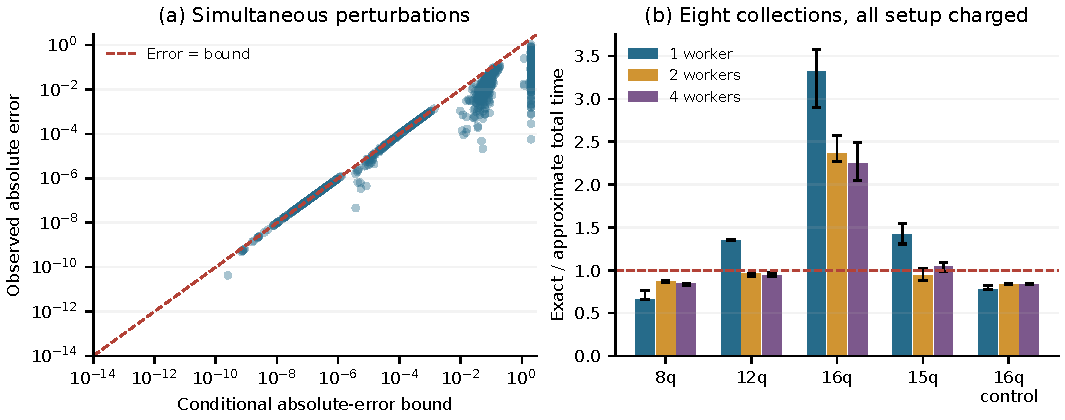
\includegraphics[width=0.98\textwidth]{figures/sensitivity_tradeoff.pdf}
\caption{Observable-sensitivity validation. (a) Actual errors versus conditional bounds for simultaneous perturbations; zero points are omitted on logarithmic axes. (b) Median eight-collection lifetime ratios, with whiskers spanning session/seed configurations rather than confidence intervals. Each ratio compares exact and approximate execution at the same worker count. Profiling, search and worker setup/shutdown are charged.}
\label{fig:sensitivity}
\end{figure*}



% Generated by benchmarks/plot_sensitivity.py from validated summary.json.
\begin{table*}[t]
\centering
\caption{Sensitivity study: ranges across three interpreter sessions and the stated seeds. Warm speedups compare exact and bounded execution at equal worker counts. Lifetime charges eight collections, profiling, search and pool setup/shutdown. Payload is the largest individual complex128 state, not RSS. Budget: $0.01$ per output.}
\label{tab:sensitivity-results}
\footnotesize
\begin{tabular}{lrrrrrrr}
\toprule
Fixture & Seeds & Workers & Width & Payload factor & Warm speedup & Lifetime speedup & Profile (ms) \\
\midrule
8q / 2 blocks & 1 & 1 & $8\to 4$ & 16 & 2.23--2.40 & 0.66--0.76 & 7.50--8.07 \\
8q / 2 blocks & 1 & 2 & $8\to 4$ & 16 & 1.58--2.64 & 0.86--0.88 & 21.80--36.20 \\
8q / 2 blocks & 1 & 4 & $8\to 4$ & 16 & 1.16--1.79 & 0.82--0.85 & 25.95--28.15 \\
12q / 2 blocks & 1 & 1 & $12\to 6$ & 64 & 4.80--5.18 & 1.35--1.35 & 11.17--13.00 \\
12q / 2 blocks & 1 & 2 & $12\to 6$ & 64 & 2.48--3.66 & 0.93--0.97 & 21.71--24.60 \\
12q / 2 blocks & 1 & 4 & $12\to 6$ & 64 & 2.46--2.84 & 0.93--0.98 & 21.76--24.11 \\
16q / 2 blocks & 3 & 1 & $16\to 8$ & 256 & 40.56--53.88 & 2.89--3.57 & 133.05--165.46 \\
16q / 2 blocks & 3 & 2 & $16\to 8$ & 256 & 27.43--31.70 & 2.27--2.57 & 87.83--103.89 \\
16q / 2 blocks & 3 & 4 & $16\to 8$ & 256 & 22.70--30.28 & 2.04--2.49 & 89.91--109.28 \\
15q / 3 blocks & 3 & 1 & $15\to 5$ & 1024 & 30.95--35.46 & 1.31--1.55 & 138.32--158.77 \\
15q / 3 blocks & 3 & 2 & $15\to 5$ & 1024 & 9.31--12.51 & 0.88--1.02 & 138.80--181.29 \\
15q / 3 blocks & 3 & 4 & $15\to 5$ & 1024 & 11.86--17.78 & 0.99--1.10 & 106.85--137.25 \\
16q connected control & 1 & 1 & $16\to 16$ & 1 & 0.92--1.03 & 0.77--0.82 & 138.56--165.83 \\
16q connected control & 1 & 2 & $16\to 16$ & 1 & 0.97--1.00 & 0.83--0.85 & 106.49--130.78 \\
16q connected control & 1 & 4 & $16\to 16$ & 1 & 0.99--1.01 & 0.83--0.84 & 108.31--126.78 \\
\bottomrule
\end{tabular}
\end{table*}


\subsection{Proof of Theorem~\ref{thm:observable-error}}
\begin{IEEEproof}
For a Pauli rotation channel $\mathcal U_g$, define $\mathcal D_g(A)=-i[P_g/2,A]$. Then $\partial_g\mathcal U_g=\mathcal D_g\mathcal U_g$ and $\partial_g^2\mathcal U_g=\mathcal D_g^2\mathcal U_g$. Since $\|P_g\|_\infty=1$,
\begin{equation}
 \|\mathcal D_g(A)\|_1\leq\|P_gA\|_1/2+\|AP_g\|_1/2\leq\|A\|_1.
\end{equation}
Every unitary channel preserves trace norm. Differentiating a circuit once or twice inserts one or two such derivative maps. This also covers two derivatives of the same occurrence. Using $\|\rho\|_1=1$ and $|\operatorname{Tr}(O_k A)|\leq\|O_k\|_\infty\|A\|_1$ therefore gives
\begin{equation}
 |\partial_g f_k(\vartheta)|\leq1,\qquad
 |\partial_g\partial_h f_k(\vartheta)|\leq1
 \label{eq:uniform-derivative-bounds}
\end{equation}
at every angle vector $\vartheta$, not only the profiled point. A structural backward cone contains every gate that can affect the evolved observable. Changing angles leaves gate supports fixed, so derivatives involving an occurrence outside $C_k$ vanish identically.

Put $q(t)=f_k(\theta+t\delta)$. Equation~\eqref{eq:uniform-derivative-bounds} implies $|q'(t)|\leq L_k$ and $|q''(t)|\leq L_k^2$. Taylor's integral identity gives
\begin{equation}
 q(1)-q(0)=J_k\delta+\int_0^1(1-t)q''(t)\,dt.
\end{equation}
Taking absolute values bounds the remainder by $L_k^2/2$. Integrating the first-derivative bound yields $L_k$, while the range of a norm-one observable yields two. Taking their minimum proves Eq.~\eqref{eq:ideal-sensitivity-bound}.

For sharpness, compose $m$ single-qubit $R_Y$ occurrences on $|0\rangle$, all at zero, and request $Z$. Perturb every occurrence by $d$. The gradient at the starting point vanishes, but the output change is $1-\cos(md)$ with $L=m|d|$. Consequently,
\begin{equation}
 \lim_{d\to0}\frac{1-\cos(md)}{(m d)^2}=\frac12.
\end{equation}
No smaller uniform coefficient can replace $1/2$ in the quadratic remainder. The same example shows why counting shared occurrences is necessary. Expanding around a total rotation of $\pi/2$ similarly saturates the linear bound to first order.

Finally, with the structural zeros enforced, $|(\widehat J_k-J_k)\delta|\leq\eta L_k$. Adding this to the Taylor term and allowing error $\eta$ at each independently evaluated endpoint proves Eq.~\eqref{eq:sensitivity-bound}. This last step is conditional on the stated numerical error bounds and exact evaluation of the bound expression itself.
\end{IEEEproof}

The theorem is an application of unitary derivative bounds and Taylor's integral remainder, not an inference from a finite sample. The two corollaries add sufficient precision and reduced-evaluation conditions for this planner. The experiments validate particular implementations and timing hypotheses; they do not establish a universal speedup or the novelty of the underlying mathematical inequalities.

\subsection{Sensitivity Reproducibility}

The implementation assumes $\eta=10^{-10}$ in the study. Independent double-precision agreement does not prove this allowance or establish outward rounding of the computed bound. The bound is consequently an analytic error-control rule with an explicit numerical assumption. The evaluated program must already be feasible; neither small gradients nor approximate candidates supply otherwise unavailable exact profiles.

\path{src/lazyqc/sensitivity.py} implements profiling and bounded candidate search. \path{benchmarks/run_sensitivity.py} defines the cases; \path{tests/test_sensitivity.py} includes independent dense-matrix and analytic regression tests. Raw final observations reside in \path{results/sensitivity/session0/} through \path{results/sensitivity/session2/}; \path{results/sensitivity/frozen_source/} contains their measured source snapshot. Pilot runs are excluded from aggregation. \path{benchmarks/summarize_sensitivity.py} validates source hashes and produces the summary; \path{docs/SENSITIVITY.md} specifies cost scopes and reproduction. Native thread counts are fixed at one on the same unpinned, heterogeneous i7-13700H host used for the local-worker study. Summed RSS includes shared pages more than once and may retain allocations from earlier exact collections.


\section{Earlier Planning Studies}
\label{app:earlier}
The studies in this appendix predate the QML evaluation. They use small QAOA-derived fixtures and compare planning policies with each other rather than with direct execution, which is why they are not part of the main results. They remain useful because they isolate the cost of search, the value of joint cut selection and the role of expected reuse.

\subsection{Two-policy selection with expected reuse}
Before the QML study, we evaluated whether historical timing can decide between independent request optimization followed by deduplication (B3) and joint group, rewrite and cut search (B5) for a declared number of collections $R\in\{1,2,4,\dots,512\}$. For each policy $p$, a reconstructed lifetime $\widetilde L_p(R)=\operatorname{median}(H_p)+R\operatorname{median}(T^{\mathrm{warm}}_p)$ combines cold planning with warm calls, and regret is measured against the cheaper of the two policies. Rules were trained on some timing repetitions and evaluated on others, separately for each workload, so the study holds out repetitions and not circuit families. Table~\ref{tab:selection_quality} shows that a history threshold makes no error on the 20 path and star decisions and four errors on 30 further decisions, while running both searches and then choosing raises the mean regret to 122\,ms, above always choosing the joint search. Obtaining an alternative can cost more than the decision saves, which is the same lesson the analysis budget encodes.

\begin{table}[!t]
\caption{Selection Against the Two-Policy Lifetime Reference. Mean Regret in Milliseconds; Training and Test Repetitions Are Separate.}
\label{tab:selection_quality}
\centering
\setlength{\tabcolsep}{2pt}
\footnotesize
\begin{tabular}{lrrrr}
\toprule
 & \multicolumn{2}{c}{Path/star: 20 decisions} & \multicolumn{2}{c}{Additional: 30 decisions}\\
\cmidrule(lr){2-3}\cmidrule(lr){4-5}
Rule & Errors & Regret & Errors & Regret\\
\midrule
Always independent & 6/20 & 76.03 & 5/30 & 21.76\\
Always joint & 14/20 & 89.33 & 25/30 & 101.09\\
History threshold & 0/20 & 0.00 & 4/30 & 16.14\\
History + execution score & 1/20 & 4.88 & 3/30 & 13.82\\
Both searches, then select & 14/20 & 122.33 & n/a & n/a\\
\bottomrule
\end{tabular}
\end{table}

\subsection{Joint grouping and exact cutting}
The historical cutting manifest contains 11 small workloads, including four-qubit QAOA path and star instances, overlapping and disjoint batches, and dense controls. B3 chooses rewrites and cuts independently per request before deduplication, while B5 chooses them jointly; both respect each case's fragment limit. Joint selection reduces unique fragment experiments from 148 to 67 on the path and from 76 to 58 on the star (Table~\ref{tab:cutting_results}), but cold joint planning loses on every feasible case, with B3/B5 total-time ratios of 0.21 to 0.59. Repeated collections of the same bound batch eventually repay the search: over 512 calls the path breaks even after 18 to 21 calls and reaches $1.59\times$ ($\approx1.45\times$ with calibration charged), while the overlapping batch repays late and the star and local-Pauli controls never do (Table~\ref{tab:cache_results}). None of these comparisons includes dense execution, which on such small circuits is faster than any cut plan: on a six-qubit QAOA path, ten dense collections took 1.06\,ms against 389\,ms for the joint cut plan.

\begin{table}[!t]
\caption{Historical Cutting Results: Unique Experiments and Warm-Cache B3/B5 Speedups (Seven Paired Trials).}
\label{tab:cutting_results}
\centering
\setlength{\tabcolsep}{3pt}
\footnotesize
\begin{tabular}{lrrcc}
\toprule
Workload & B3 & B5 & Reduction & Speedup [95\% CI]\\
\midrule
QAOA path & 148 & 67 & 54.7\% & $1.26\times$ [1.08--1.45]\\
QAOA star & 76 & 58 & 23.7\% & $1.74\times$ [1.24--2.51]\\
Overlapping batch & 8 & 1 & 87.5\% & $1.36\times$ [1.21--1.57]\\
Disjoint cones & 8 & 8 & 0.0\% & $1.00\times$ [0.91--1.11]\\
\bottomrule
\end{tabular}
\end{table}

\begin{table}[!t]
\caption{Amortized Joint-Planning Speedups and Break-Even Calls over 512 Collections (Three Sessions).}
\label{tab:cache_results}
\centering
\setlength{\tabcolsep}{3pt}
\footnotesize
\begin{tabular}{lccc}
\toprule
Workload & Speedup & Break-even & With calibration\\
\midrule
QAOA path & $1.59$--$1.60\times$ & 18--21 & $\approx1.45\times$\\
Overlapping batch & $1.14$--$1.29\times$ & 220--353 & $1.04$--$1.08\times$\\
QAOA star & $0.95$--$0.98\times$ & not reached & $0.96$--$0.99\times$\\
Local Pauli batch & $0.64$--$0.68\times$ & not reached & $0.73$--$0.77\times$\\
\bottomrule
\end{tabular}
\end{table}

\subsection{Earlier structural replay}
An earlier replay study reused group and cut choices across eight random bindings of the QAOA path and star circuits. Replay planning took 4.25 to 9.90\,ms against 29.80 to 249.80\,ms for fresh planning, with and without ZX rewrites, and every replayed output matched an independent NumPy reference within $5\times10^{-16}$. The stored summaries are fifth order statistics of eight bindings rather than conventional medians, and the template acquisition was not charged, so we only use these values as motivation for the charged QML replay study of Section~\ref{sec:rq3}.


\section{Local Multiprocessing}
\label{app:parallel}
\subsection{Detailed Local Multiprocessing Study}
We extend the worker study to ten predefined workloads, three separate interpreter sessions on the same i7-13700H host, and one, two, or four worker processes. Each scientific runtime uses one thread. The operating system schedules processes across the allowed 20 logical CPUs; individual cores are not pinned, and this is not an isolated host. Within each workload, every policy executes the same experiment graph and reconstruction formulas, verified by a graph fingerprint. This isolates execution-policy effects from changes in plan quality.

Nine workloads contain independent components with seeded $R_Y$, $R_Z$, and nearest-neighbor CX layers. Widths range from four to 16 qubits, component counts from two to eight, and depths from four to 80 layers. A separate connected 16-qubit circuit joins two eight-qubit components with one CX and applies noncommuting terminal rotations; its exact cut plan contains 12 fragment tasks. Independent NumPy state-vector operations validate every collection. The reference is factorized only for the explicitly independent components and simulates all 16 qubits for the bridge case. This expands numerical coverage beyond the previous same-graph worker consistency check.

For each configuration, the first collection is recorded separately, followed by nine repetitions. Parent-side per-task diagnostic executions precede these collections, so ``first'' does not denote an uninitialized interpreter. Serial, forced parallel, and automatic-dispatch modes are interleaved in randomized order within a pool configuration; configuration and workload order vary across sessions. The study records 2,052 warm timed collections and 2,310 validated collections including first calls and separate resource probes. Maximum absolute error is $3.04\times10^{-15}$. Construction, cold planning, calibration, full pool warmup, shutdown, serialized recipe sizes, and execution phases are recorded separately. Detailed workload results are in Table~\ref{tab:local_parallel_full}.

\begin{figure*}[!t]
\centering
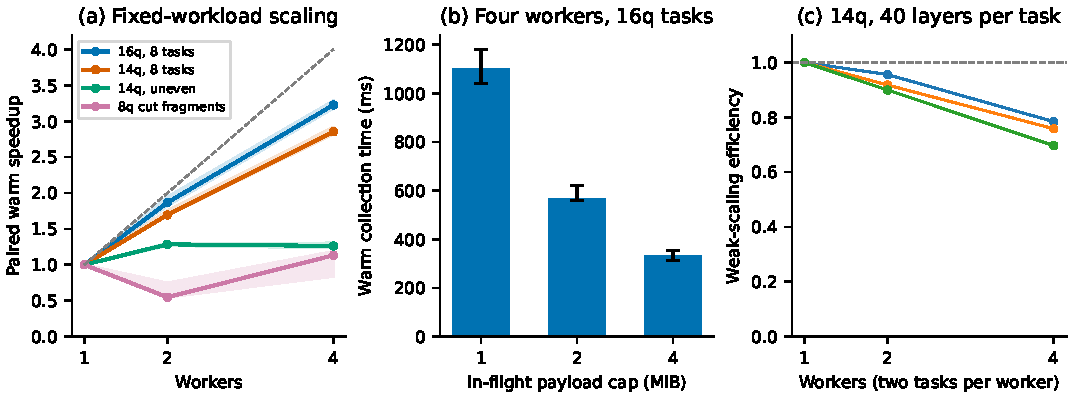
\includegraphics[width=\textwidth]{figures/local_parallel_scaling.pdf}
\caption{Measured local multiprocessing. (a) Fixed-workload speedups: lines show medians of three session-level paired geometric means; bands show their ranges, and the dashed line is ideal worker-count scaling. (b) Eight 16-qubit tasks on four workers under different aggregate payload caps: bars show medians of session medians, with session ranges. (c) Weak scaling holds two 14-qubit, 40-layer tasks per worker; each line is one session. All timings are warm and exclude setup.}
\label{fig:local_parallel_scaling}
\end{figure*}

\subsubsection{Strong Scaling and Task Granularity}
For each parallel policy, warm speedup is the geometric mean of paired serial/parallel time ratios; efficiency divides that speedup by the worker count. On eight 16-qubit components, four workers achieve $3.18\times$--$3.28\times$ speedup, corresponding to 79.6\%--82.1\% efficiency. Parallel median time is 313--355\,ms, while the separate one-worker configuration takes 1,028--1,169\,ms. The speedup uses paired serial controls within each pool configuration, so it need not equal the ratio of these independently summarized medians.

Eight balanced 14-qubit components reach $2.82\times$--$2.91\times$ on four workers. With only two components, four workers yield $1.68\times$--$1.71\times$: additional workers cannot create more independent tasks. An uneven eight-component batch, with seven four-layer components and one 80-layer component, yields only $1.24\times$--$1.30\times$. Its largest task limits completion time. Four-qubit components regress to $0.28\times$--$0.51\times$, while the connected bridge's cut fragments yield $0.84\times$--$1.19\times$. Thus the strongest scaling result concerns substantial independent tasks, not a demonstrated acceleration of connected-circuit cutting.

\subsubsection{Weak Scaling}
With two 14-qubit, 40-layer components per worker, the task count rises from two to eight as the worker count rises from one to four. Define weak-scaling efficiency as $T_1(2)/T_P(2P)$, using session median times. Four-worker efficiency is 69.7\%--78.4\%, and throughput grows from 29.7--32.4 to 90.0--93.5 tasks/s. The sublinear gain reflects the measured executor and shared host; it does not establish scaling beyond four processes.

\subsubsection{Setup Repayment and Time Allocation}
To assess short lifetimes, we sum the recorded first call and nine warm calls, adding construction, cold planning, and calibration once to both policies, plus full pool warmup and shutdown to parallel execution. This is cost accounting from interleaved observations, not a separately timed contiguous ten-call application. Full calibration takes 705--904\,ms per session; for the eight-task 16-qubit case, planning takes 210--343\,ms and four-worker warmup takes 103--146\,ms.

The 16-qubit workload retains a $2.56\times$--$2.63\times$ ten-call speedup with these charges, crossing break-even on the first recorded call in all three sessions. Eight balanced 14-qubit tasks retain $1.72\times$--$1.80\times$. In contrast, the shallow 14-qubit batch needs nine or ten calls to cross and ends at $1.00\times$--$1.02\times$; the ten-qubit batch remains slower despite its $1.19\times$--$1.25\times$ warm speedup. No later repayment is inferred for cases that do not cross within the observed horizon.

\begin{figure}[!t]
\centering
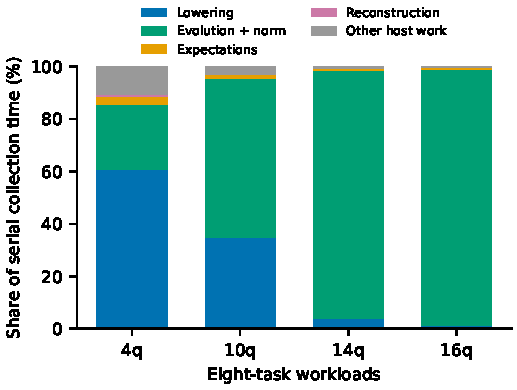
\includegraphics[width=\columnwidth]{figures/local_parallel_phases.pdf}
\caption{Time allocation in the one-worker configuration: mean per-call phase fractions over 27 warm observations per workload. Evolution includes initialization and norm checking. The residual includes host dispatch, cleanup, and instrumentation. These are serial wall-time fractions; parallel worker phase sums are not additive parent wall-time components.}
\label{fig:local_parallel_phases}
\end{figure}

Figure~\ref{fig:local_parallel_phases} explains the granularity dependence. Evolution and norm checking occupy approximately 25.0\% of serial collection time for the four-qubit workload, 60.9\% at ten qubits, 94.7\% at 14 qubits, and 98.0\% at 16 qubits. Native circuit lowering accounts for 60.8\% at four qubits. These workloads vary in depth as well as width, so the fractions characterize the tested configurations rather than a width-only law. Forced parallel execution avoids automatic-policy scoring, whose overhead remains visible: on the balanced eight-task 14-qubit workload, automatic dispatch achieves $2.58\times$--$2.62\times$, below forced parallelism.

\subsubsection{Memory, CPU, and Transport Costs}
For uniform independent tasks with payload $b$, worker count $P$, and aggregate payload budget $B$, at most $\min(P,\lfloor B/b\rfloor)$ tasks can be in flight, also bounded by available tasks. The 16-qubit states occupy 1\,MiB each. Holding four workers and the graph fixed, budgets of one, two, and four MiB yield speedups of $0.99\times$--$1.01\times$, $1.87\times$--$1.93\times$, and $3.18\times$--$3.28\times$, respectively (Fig.~\ref{fig:local_parallel_scaling}b). Provisioned processes alone do not supply usable parallelism when the payload budget serializes dispatch.

Resource measurements run in separate diagnostic collections to avoid sampling overhead in the timing trials. A 2\,ms target-period sampler reads Linux process RSS and CPU counters for the parent and the active pool. Summed sampled RSS counts shared pages once per process and may miss short peaks; it is neither unique physical memory nor an enforced RSS bound. CPU counters have 10\,ms resolution, so utilization ratios for probes shorter than 100\,ms are omitted.

For the eight-task 16-qubit workload, sampled parent-plus-pool RSS is 276--308\,MiB with four workers, compared with 147--174\,MiB serially, despite the much smaller four-MiB state-payload budget. Diagnostic CPU use is 1.29--1.38 CPU-s with four workers versus 1.04--1.14 CPU-s serially; lower latency does not imply less CPU work. The four-worker probes average approximately 3.85--4.01 CPU cores, including parent overhead. The four-worker pool still occupies roughly 276--308\,MiB when the payload cap is tightened, showing that payload throttling does not remove process overhead (Table~\ref{tab:local_parallel_resources}).

The eight 16-qubit task descriptions serialize to about 429\,KiB per collection before multiprocessing framing; results are scalar values and execution statistics. These are measured serialized object sizes, not monitored transport traffic. Numerical statevectors remain inside their executing process. The results therefore quantify a local multiprocessing trade-off among task granularity, available concurrency, setup repayment, and process footprint; they make no claim about networked or physical-QPU distribution.


% Generated by benchmarks/export_local_parallel_tables.py; do not hand-edit rows.
\subsection{Expanded Local Multiprocessing Artifacts}
The expanded study uses \path{benchmarks/run_local_parallel.py} with nine repetitions and
session indices zero through two. Raw data, plans, reference values, process samples, and source
fingerprints are in \path{results/local_parallel/session0/} through
\path{results/local_parallel/session2/}. The checked aggregate is
\path{results/local_parallel/summary.json}; its generator verifies source and graph
fingerprints. Workloads are fixed across sessions. Full calibration is charged to each workload
when calculating a standalone ten-call lifetime, although the measurement runner performs
calibration once per session. First-call and warm measurements are interleaved with controls;
unmeasured gaps are excluded from the summed cost model.

Table~\ref{tab:local_parallel_full} retains all ten workloads. $T_1$ and $T_4$ are ranges of
configuration-level median collection times. $S_2$ and $S_4$ are ranges of paired geometric-mean
speedups against serial controls measured within the corresponding pool configuration. $L_4$
includes common construction, planning, and calibration, plus parallel warmup, ten collections,
and shutdown. Bootstrap intervals for the nine paired trials in each session are retained in the
JSON, rather than conflated with session ranges. Three sessions on one host do not establish
between-machine uncertainty.

\begin{table*}[!t]
\caption{All Local Multiprocessing Workloads: Warm Timings, Paired Speedups, and Ten-Call
Setup-Charged Speedups. Ranges Span Three Sessions.}
\label{tab:local_parallel_full}
\centering
\footnotesize
\setlength{\tabcolsep}{4pt}
\begin{tabular}{lrrrrrrr}
\toprule
Workload & Tasks & $T_1$ (ms) & $T_4$ (ms) & $S_2$ & $S_4$ & $S_4/4$ & $L_4$ \\
\midrule
4q, 4 layers & 8 & 0.44--1.27 & 1.88--2.12 & 0.17--0.20 & 0.28--0.51 & 0.07--0.13 & 0.83--0.84 \\
10q, 20 layers & 8 & 9.95--11.27 & 8.93--10.76 & 0.83--0.88 & 1.19--1.25 & 0.30--0.31 & 0.89--0.91 \\
14q, 40 layers & 2 & 61.66--67.36 & 36.33--39.29 & 1.59--1.72 & 1.68--1.71 & 0.42--0.43 & 1.09--1.10 \\
14q, 40 layers & 4 & 114.50--130.81 & 39.18--42.63 & 1.63--1.74 & 2.76--2.91 & 0.69--0.73 & 1.38--1.50 \\
14q, 40 layers & 8 & 231.59--276.39 & 85.59--88.85 & 1.69--1.75 & 2.82--2.91 & 0.71--0.73 & 1.72--1.80 \\
16q, 40 layers & 8 & 1027.70--1168.86 & 312.80--355.16 & 1.82--1.94 & 3.18--3.28 & 0.80--0.82 & 2.56--2.63 \\
14q, 4 layers & 8 & 26.72--29.94 & 11.38--13.56 & 1.29--1.47 & 2.23--2.34 & 0.56--0.58 & 1.00--1.02 \\
14q, 80 layers & 8 & 452.12--474.31 & 159.90--162.88 & 1.71--1.74 & 2.73--3.03 & 0.68--0.76 & 1.84--2.08 \\
14q, uneven depths & 8 & 79.40--99.32 & 63.71--77.81 & 1.27--1.30 & 1.24--1.30 & 0.31--0.33 & 0.99--1.04 \\
8q cut fragments & 12 & 7.33--7.96 & 8.15--11.58 & 0.55--0.75 & 0.84--1.19 & 0.21--0.30 & 0.86--0.91 \\
\bottomrule
\end{tabular}
\par\vspace{8pt}
\caption{Resource Diagnostics for Eight 16-Qubit Tasks. Each State Occupies 1 MiB; Values Span
Three Separate Profiling Collections, One per Session.}
\label{tab:local_parallel_resources}
\centering
\footnotesize
\setlength{\tabcolsep}{5pt}
\begin{tabular}{rrrrrr}
\toprule
Workers & Payload cap (MiB) & Warm time (ms) & Sampled RSS sum (MiB) & CPU-s & Mean cores \\
\midrule
1 & 1 & 1027.70--1168.86 & 147.3--173.9 & 1.04--1.14 & 0.99--1.01 \\
2 & 2 & 562.61--654.97 & 213.4--239.0 & 1.19--1.61 & 2.03--2.10 \\
4 & 1 & 1039.75--1180.83 & 277.1--307.0 & 1.15--1.44 & 1.09--1.12 \\
4 & 2 & 558.94--622.99 & 276.3--307.6 & 1.14--1.67 & 2.07--2.13 \\
4 & 4 & 312.80--355.16 & 276.2--307.7 & 1.29--1.38 & 3.85--4.01 \\
\bottomrule
\end{tabular}
\end{table*}

The uneven case contains seven four-layer components and one 80-layer component. Other uncut
rows use the same depth per component. The cut row joins two eight-qubit, 20-layer components
with a CX bridge and adds terminal rotations. Scalar observables are validated using an
independent NumPy implementation; no sampled quantum execution is involved.

Warm timings in Table~\ref{tab:local_parallel_resources} come from unprofiled trials. RSS and
CPU columns come from separate instrumented collections. RSS is the sampled sum over the parent
and the active pool, including shared-page double counting and retained runtime allocations.
CPU-s sums user and system process counters; mean cores divides that CPU time by profiled
collection wall time and includes sampler/parent overhead. Raw process counters have 10 ms
resolution. All reported resource probes in this table exceed 100 ms; shorter workloads retain
raw counters but suppress derived utilization ratios. These measurements do not bound peak RSS
or measure energy.


\section{Artifacts and Provenance}
\label{app:provenance}
All raw observations, manifests and runners are part of the accompanying repository. The planner-versus-direct study is defined by \path{benchmarks/direct_baseline_manifest.json}. Its runners are \path{benchmarks/run_direct_baselines.py}, \path{benchmarks/run_gradient_baselines.py} and \path{benchmarks/run_memory_wall.py}, which share \path{benchmarks/direct_support.py}, and \path{benchmarks/summarize_direct.py} recomputes every reported median, ratio and figure from the raw rows in \path{results/direct/}. The GPU runners declare their dependencies inline, pinned by adjacent script lockfiles, and can be reproduced with \texttt{uv run --locked --script}. The same-backend comparison is \path{results/direct/backend_matrix.json}. The cloud confirmation ran \path{cloud/gpu-baselines.yaml} through \path{scripts/sky_gpu.sh} on a Lambda \texttt{gpu\_1x\_h100\_pcie} instance for 2\,h\,23\,min, and its results, including the host's \texttt{nvidia-smi} and \texttt{lscpu} records, are in \path{results/direct/remote/nvidia-h100-pcie/}. Each result file records the manifest hash, a hash of the package and runner sources, the command line, the thread settings, the CPU and GPU models and the package versions.

The QML matrix, the exhaustive grouping reference, the replay and parallel probes and the external backend pilots are in \path{results/qml_workloads/}, produced by the corresponding \path{benchmarks/run_qml_*.py}, \path{run_grouping_oracle.py}, \path{run_ionq_*.py} and \path{run_iqm_qml_*.py} runners and frozen in \path{benchmarks/qml_workload_manifest.json}. The interleaved comparison of the pre-study and current planners used in RQ3 is \path{results/qml_workloads/planner_ab/}, recomputed by \path{benchmarks/compare_planner_versions.py}; an earlier rerun in \path{results/qml_workloads/v2/} ran right after sustained GPU load, shows a uniform slowdown of its collections, and is not used. The analysis-budget coefficients are fitted by \path{benchmarks/calibrate_analysis_budget.py}, with its output in \path{results/analysis_budget/calibration.json}, and the Hamiltonian-averaging study of the budget is \path{results/analysis_budget/hamiltonian.json}, produced by \path{benchmarks/run_analysis_budget.py}. The earlier planning studies of Appendix~\ref{app:earlier} are in \path{results/p4_p5/}, \path{results/priorities/} and \path{results/workload_manifest/v2/}, with their analysis in \path{paper/analysis/}.

The generalization studies of Section~\ref{sec:generalization} are frozen in \path{benchmarks/qml_heldout_family_manifest.json}, \path{benchmarks/grouping_oracle_heldout_manifest.json}, \path{benchmarks/trained_iris_qml_v3_manifest.json} and \path{benchmarks/fourier_trained_qml_manifest.json}. The held-out screen runs as two sessions of \path{benchmarks/run_qml_depth_screen.py} and is summarized by \path{benchmarks/summarize_heldout_families.py}, which applies the analysis plan recorded in its manifest and checks the manifest hash of every session. The trained models come from \path{benchmarks/run_trained_iris_qml.py} and, for the replayed classifiers, \path{benchmarks/export_fourier_trained_models.py} followed by \path{benchmarks/run_fourier_trained_qml.py}. The exporter rebuilds every test split with the original study's code and refuses to continue unless its hash matches the one that study recorded. The tied-parameter control is \path{benchmarks/run_tied_qml_gradients.py}. The matched-basis IQM probes are \path{results/qml_workloads/iqm_garnet_basis_probe.json} and \path{results/qml_workloads/iqm_garnet_basis_probe_line.json}, produced by \path{benchmarks/run_iqm_qml_basis_probe.py} and summarized by \path{benchmarks/summarize_iqm_basis_probe.py}. \path{benchmarks/paper_generalization_tables.py} regenerates the corresponding tables from these results.

The revised beyond-device-memory study is defined by the \texttt{memory\_wall} section of \path{benchmarks/direct_baseline_manifest.json}. \path{benchmarks/run_memory_wall.py} now records exact global-MPS, reused-circuit tensor-network, LazyQC CPU and LazyQC GPU-placement timings, cone-width ranges, bond dimensions, validation errors, source hashes and environment fingerprints in \path{results/direct/memory_wall.json}. \path{benchmarks/summarize_direct.py} regenerates Tables~\ref{tab:memory-wall} and~\ref{tab:intermediate-cones} and their Markdown summaries from those rows. The direct Qiskit LightCone studies are frozen in \path{benchmarks/lightcone_ablation_manifest.json} and \path{benchmarks/lightcone_jacobian_manifest.json}, with runners \path{benchmarks/run_lightcone_ablation.py} and \path{benchmarks/run_lightcone_jacobian_ablation.py}. Their raw observations are \path{results/direct/lightcone_ablation.json} and \path{results/direct/lightcone_jacobian_ablation.json}; \path{benchmarks/summarize_lightcone_ablation.py} regenerates Table~\ref{tab:lightcone-ablation}. The policy comparison in Table~\ref{tab:policy-ablations} is a post-hoc analysis of the two frozen held-out session files, with no new timings: \path{benchmarks/summarize_policy_ablations.py} regenerates \path{results/qml_workloads/policy_ablations.json}, its Markdown report and the LaTeX table.

No immutable public release identifier is associated with these measurements yet.


\bibliographystyle{IEEEtran}
\bibliography{references}

\end{document}
